\documentclass[11pt]{article}

\usepackage[margin=1in]{geometry}
\usepackage{graphicx}
\usepackage{booktabs}
\usepackage{hyperref}
\usepackage{url}
\usepackage{amsmath}
\usepackage{amssymb}
\usepackage{authblk}
\usepackage{microtype}
\usepackage{caption}
\usepackage{subcaption}
\usepackage{float}
\usepackage[dvipsnames]{xcolor}
\usepackage{enumitem}
\usepackage{parskip}

\hypersetup{
  colorlinks=true,
  linkcolor=NavyBlue,
  citecolor=NavyBlue,
  urlcolor=NavyBlue,
}

\title{\vspace{-2em}Human Drawing Structure as Priors for Abstract Reasoning:\\
A Decomposition of CogARC Trajectories into Error Types, Chunks,
Strategies, and Common-Error Signals}

\author[1]{Author Name\thanks{Correspondence: \texttt{author@example.com}}}
\affil[1]{Affiliation}
\date{\today}

\begin{document}

\maketitle

\begin{abstract}
We analyse 14{,}107 human drawing trajectories from the CogARC
behavioural release (75 tasks, 233 Experiment-2 subjects) with a view
to extracting priors that a graph-neural-network ARC solver can
consume. We decompose each trajectory into (i) motor slips vs
cognitive errors using timing, spatial and rule-alignment signals;
(ii) pause-segmented chunks that correspond to self-defined cognitive
units; and (iii) a best-matching canonical drawing strategy drawn
from six interpretable baselines (object-first, color-first, nearest-
neighbour color-first, row-first, column-first, random-3). We then
ask whether humans follow a single canonical strategy per task
(they do not), whether task-intrinsic features predict strategy
choice (they do, with Spearman $\rho \in 0.3\text{--}0.6$), whether
chunks diagnose which common error a participant commits (only on
task pairs with no majority-class dominance), and whether being
error-prone is a personal trait (yes, split-half $\rho = +0.35$)
as distinct from being prone to a \emph{specific} common error
(no, $\rho \leq 0.16$). Variance decomposition shows task identity
explains 4--5$\times$ more of each error outcome than subject
identity does, and early chunks (first 25\% of the trajectory)
predict the participant's final Top-Error at 74\% accuracy on
balanced pairs --- a useful online signal. We discuss how these
findings translate into task-conditional graph priors for an ARC
GNN.
\end{abstract}


\section{Introduction}
\label{sec:intro}

The Abstraction and Reasoning Corpus (ARC) \cite{chollet2019measure}
presents pairs of input/output grids and requires a system to infer
the underlying transformation. While the benchmark is usually framed
as a symbolic program-synthesis problem, a growing literature argues
that \emph{how humans produce the answer} --- their order of edits,
which objects they draw first, how they pause, and which wrong
answers they commonly converge on --- is informative data for the
priors and search policies that a machine solver might use.

CogARC \cite{cogarc2024} provides the first large-scale behavioural
release on ARC: 49 Experiment-1 subjects in fixed task order and
233 Experiment-2 subjects in randomised task order, drawing on 75
tasks with complete edit-by-edit trajectories (time-stamped pen
strokes, reaction times per edit, reset/show-example interface
events, and the final submitted grid). Each task also carries a
canonical set of label grids: the correct \texttt{Success} answer
and the most common wrong answers \texttt{Top Error 1},
\texttt{Top Error 2}, \texttt{Top Error 3}$\ldots$ (abbreviated TE1,
TE2, TE3 throughout).

Our target consumer is an ARC-GNN solver that produces
multiple candidate ``prior graphs'' per task
(object-level, color-adjacency, hierarchical, row/column, stamp, and
others) and learns to weight them. Our goal is to identify
\emph{which priors} the GNN should up-weight on \emph{which tasks}
and to separate \emph{consistent human structure} from noise in
the behavioural data. To that end we build a pipeline of five
analyses on the CogARC Experiment-2 release (\S\ref{sec:motor}
through \S\ref{sec:errors}) and end with a discussion of what the
results imply for GNN priors (\S\ref{sec:gnn}).

\paragraph{Contributions.}
\begin{enumerate}[leftmargin=*, topsep=2pt, itemsep=1pt]
  \item A motor-vs-cognitive per-edit classifier combining five
        signals (spatial distance, quick-correction bursts, reaction-
        time $z$-score, match to known Top-Error grids, wrong-run
        membership) with split-half Spearman reliability
        $\rho = 0.93$ motor / $\rho = 0.98$ cognitive across 75
        tasks (\S\ref{sec:motor}).
  \item A chunk pipeline that segments each trajectory by pauses
        ($\max(2\cdot\text{median rt}, 500\,$ms$)$) and computes
        per-chunk structural features (size, color homogeneity,
        connectedness, IoU with Success components and color
        classes). Pooled over 75 tasks $\times$ 233 subjects the
        chunks reveal a \emph{color$\,\succ\,$spatial$\,\succ\,$axis}
        hierarchy: 86\% single-color, 69\% 4-connected, 37\% axis-
        aligned, 6\% on a diagonal, 17\% span multiple connected
        components while remaining single-color
        (\S\ref{sec:chunks}).
  \item A comparison of human chunks against six canonical synthetic
        strategies (\S\ref{sec:strategies}). No single strategy
        dominates; humans match different strategies on different
        tasks.
  \item A task-level predictor analysis
        (\S\ref{sec:taskpredictors}) that identifies what task
        features drive strategy choice \emph{without} using
        unreliable Obj/Geo/Num/GoD tags.
        \texttt{n\_success\_cc}, \texttt{n\_colors\_output},
        \texttt{mean\_cc\_area}, \texttt{n\_reset\_mean} and
        \texttt{symmetry\_h} produce interpretable Spearman
        correlations $\rho \in [0.30, 0.58]$ with the subject-usage
        share of individual strategies.
  \item A chunk-based common-error diagnostic
        (\S\ref{sec:errors}): early chunks (first 25\%) predict the
        participant's Top-Error at 74\% on balanced pairs ---
        $+18.5$ percentage points above majority baseline --- but
        class imbalance (TE1 is $\sim$60\% of errors) masks the
        signal on TE1-vs-other comparisons. Error-\emph{prone} is a
        stable personal trait; which specific error is not.
\end{enumerate}


\section{Data and preprocessing}
\label{sec:data}

\paragraph{CogARC release.}
We use the Zenodo 18177487 release \cite{cogarc2024}: 75 tasks,
Experiment-1 (49 subjects, fixed order), Experiment-2 (233 subjects,
randomised order; order of trials is \emph{not} exposed in the
release). Each trajectory is a CSV of \{\texttt{action, x, y, color,
time, rt}\} rows. Actions include \texttt{edit}, \texttt{reset},
\texttt{showex}, \texttt{hideex}, \texttt{copy}, \texttt{submit}.
For each task and subject we reconstruct the ordered edit sequence
and the final submitted grid (\texttt{submission1.json}).

\paragraph{Targets.}
For every task the release provides \texttt{Success} plus several
\texttt{Top Error $k$} grids enumerating the most common wrong
submissions across participants. We match a participant's submission
against these grids by exact equality; unmatched submissions are
labelled \texttt{Other}.

\paragraph{Chunking.}
A \emph{chunk} is a maximal run of consecutive edits with
inter-edit reaction time below the per-trajectory pause threshold
$\max(2 \cdot \tilde{\text{rt}}, 500\,\text{ms})$, where
$\tilde{\text{rt}}$ is the subject's median reaction time on the
trajectory. Each chunk is characterised by size, number of distinct
cells touched, color homogeneity
$= \max_c \#\{e\in \text{chunk}:\text{color}(e){=}c\} / |\text{chunk}|$,
whether its cells form a single 4-connected component, its
bounding-box footprint, best IoU against any 4-connected Success
component, and best IoU against any Success color class.


\section{Motor slips vs cognitive errors}
\label{sec:motor}

\subsection{Classification}

We classify each \emph{wrong} edit (edit whose (color, position)
does not match the Success grid) as \texttt{motor},
\texttt{cognitive}, or \texttt{ambiguous}. Five signals contribute:

\begin{enumerate}[leftmargin=*, topsep=2pt, itemsep=1pt]
  \item \textbf{Spatial distance} to nearest correct
        same-color cell (Chebyshev). A motor slip is typically 1
        cell off.
  \item \textbf{Quick correction burst}: the edit is undone or
        overwritten within 2~s or 3 later edits.
  \item \textbf{Reaction-time $z$-score} computed within the
        subject's trajectory. Slow outliers ($z > 1.5$) suggest
        deliberation, not slip.
  \item \textbf{Matches a known Top Error grid} at the edit's
        cell with the Top-Error-specified color.
  \item \textbf{Membership in a wrong-run}: consecutive wrong
        edits in a region. Runs argue for a coherent wrong plan.
\end{enumerate}

The five signals are combined with simple rules: an edit is
\texttt{motor} if spatial distance $\leq 1$ AND (quick correction OR
NOT cognitive-flag), and \texttt{cognitive} otherwise unless RT
$z$-score and distance both look slip-like, in which case
\texttt{ambiguous}.

\subsection{Reliability and buckets}

Across all 75 tasks we compute per-trajectory motor- and cognitive-
rates and per-task averages. Split-half Spearman reliability
across random subject halves gives $\rho_{\text{motor}} = 0.93$
and $\rho_{\text{cognitive}} = 0.98$: the task ordering is highly
robust. Tasks fall into three buckets using \texttt{motor\_rate}:

\begin{itemize}[leftmargin=*, topsep=2pt, itemsep=1pt]
  \item \textbf{motor-dominant} (\texttt{motor\_rate} $\geq 0.20$,
        10 tasks): participants mostly slip; wrong edits cluster on
        the 1-cell neighbourhood of correct cells.
  \item \textbf{mixed} (\texttt{motor\_rate} $\in [0.05, 0.20)$,
        20 tasks).
  \item \textbf{cognitive-dominant} (\texttt{motor\_rate} $< 0.05$,
        45 tasks): participants execute coherent but wrong plans.
\end{itemize}

Figure \ref{fig:motor} summarises the classifier: reaction-time
distributions, per-task rate ordering with bootstrap 95\% CIs,
example trajectories in each regime, and split-half reliability.
Figure \ref{fig:motor-case} shows six concrete tasks (three per
bucket) with Success, test input, and exemplar subject trajectories.

\begin{figure}[H]
  \centering
  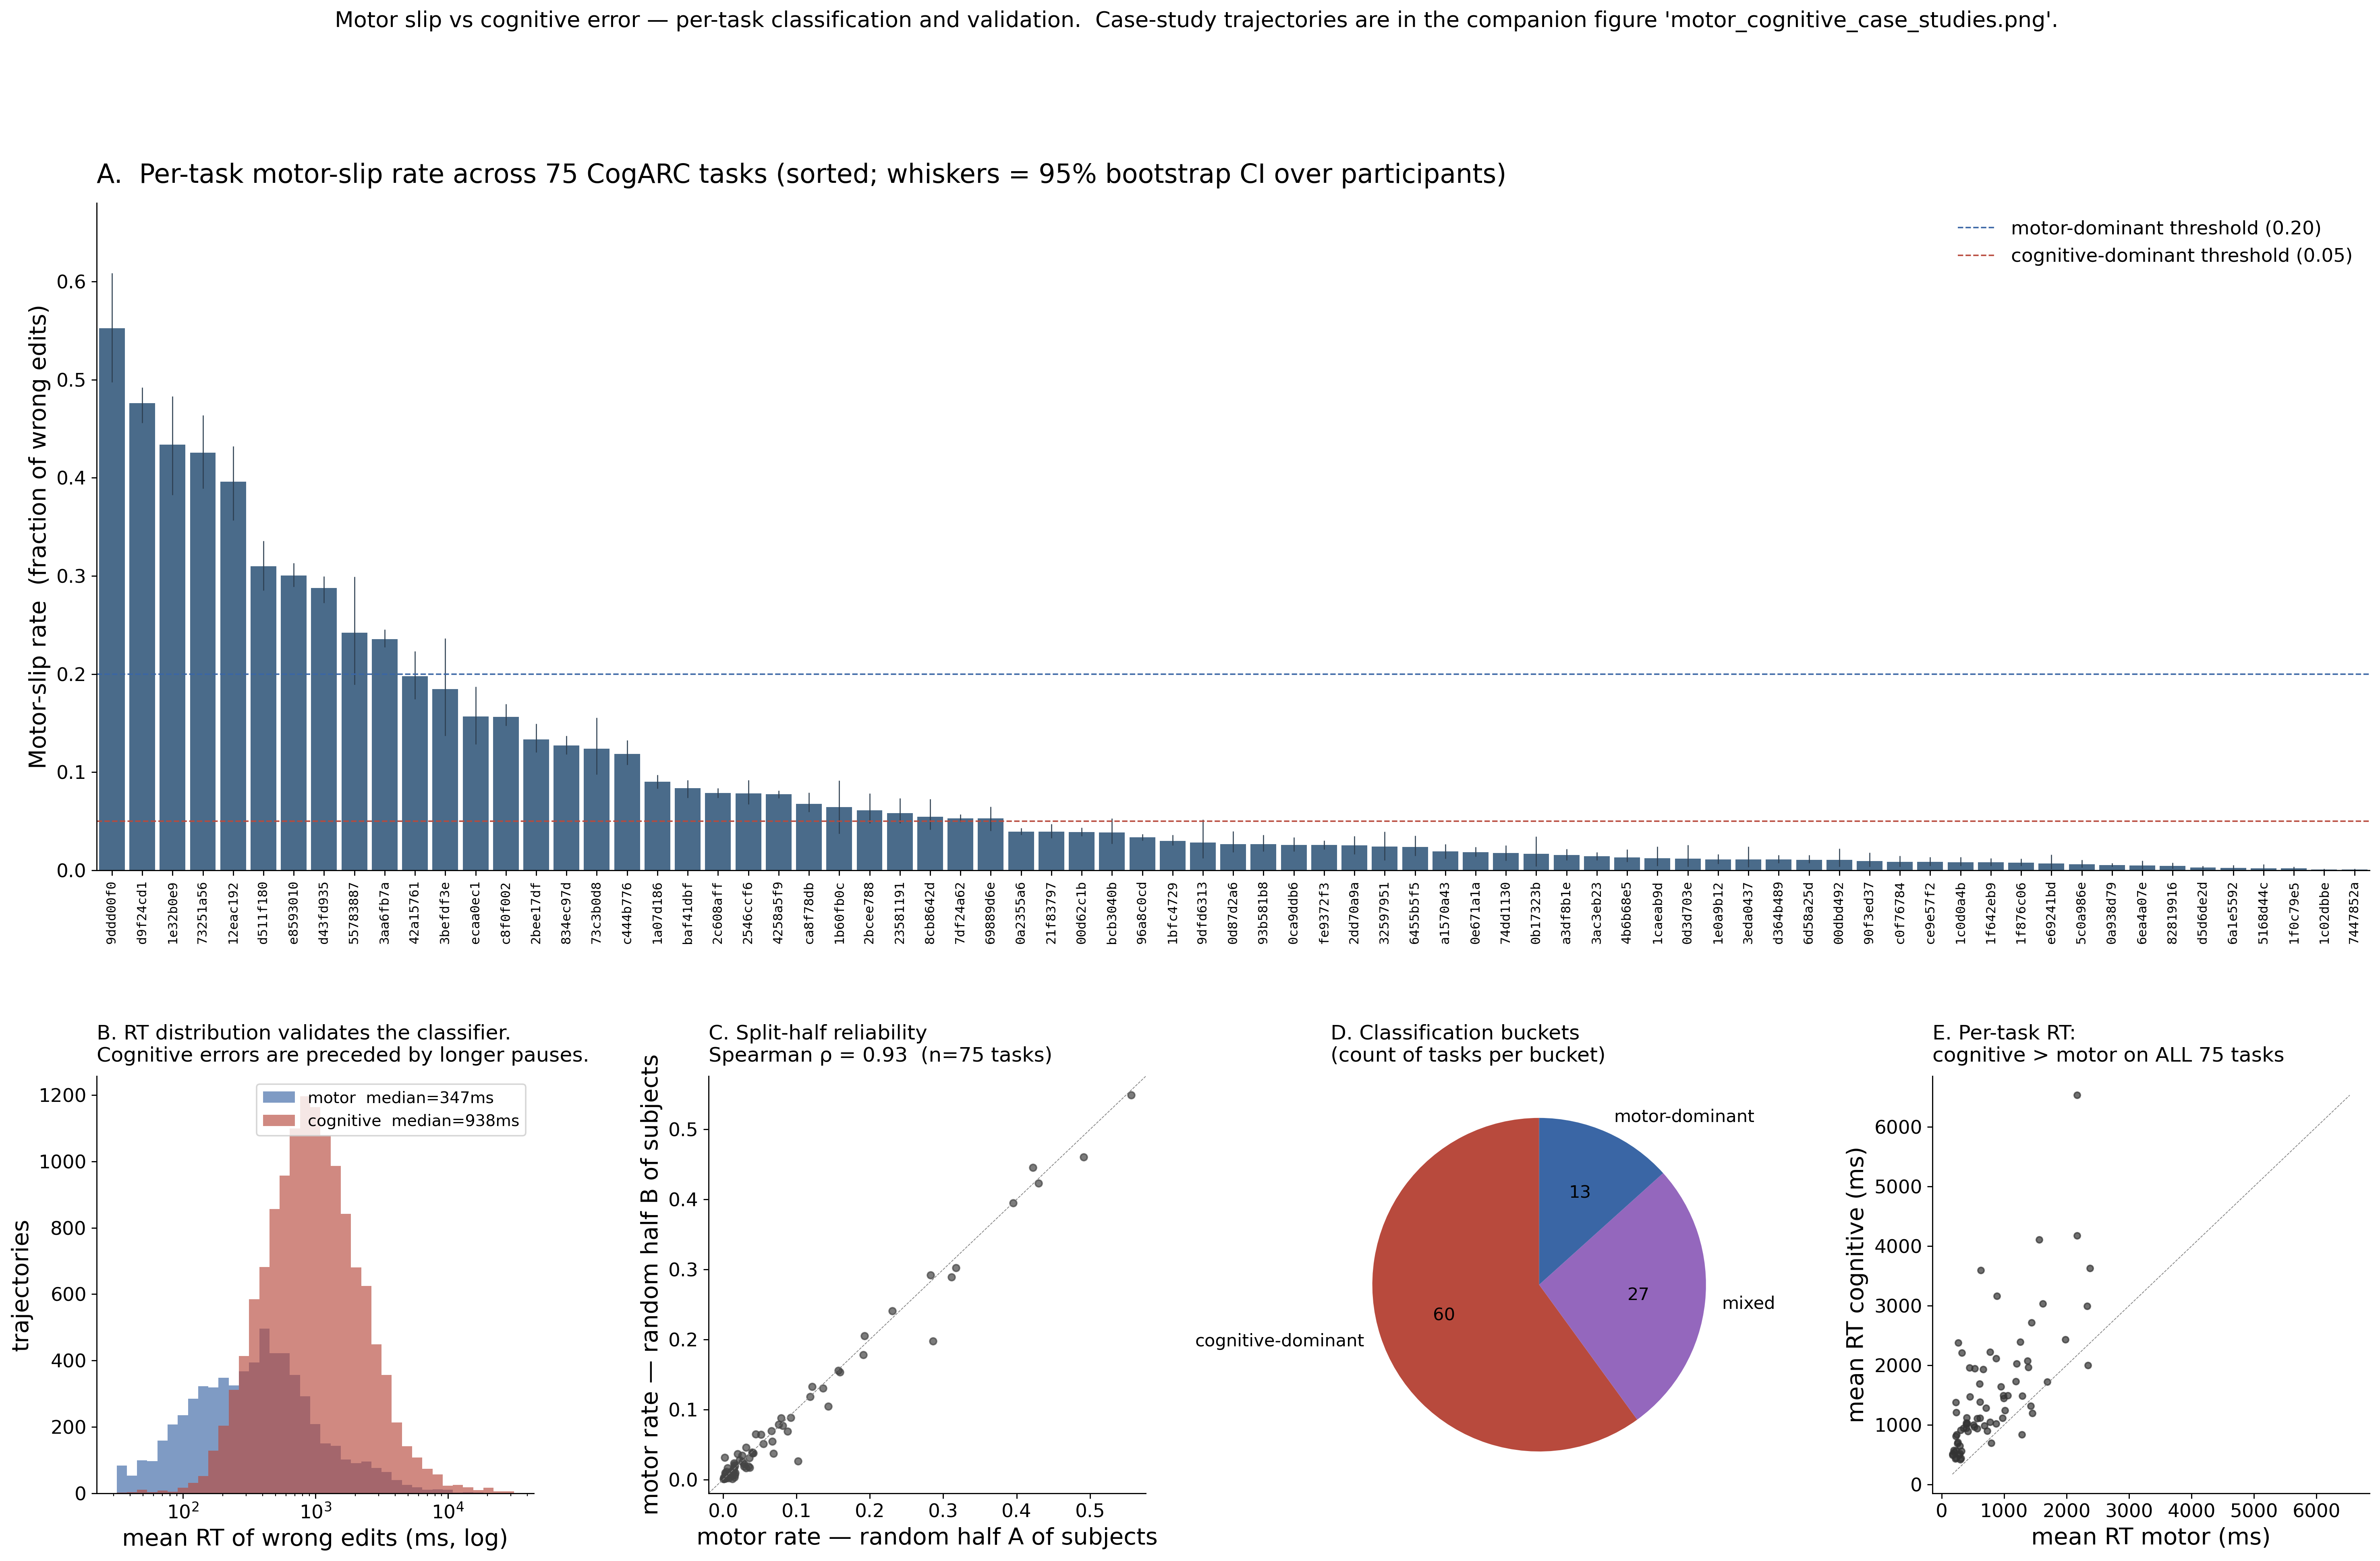
\includegraphics[width=\linewidth]{figures/motor_vs_cognitive_figure.png}
  \caption{Motor slips vs cognitive errors. Top row: RT
  distributions per class, per-task rates with bootstrap CIs,
  split-half reliability. Bottom row: case study trajectories in
  motor-dominant (green) and cognitive-dominant (red) tasks.
  Cutoffs \texttt{motor\_rate} $\geq 0.20$ for motor-dominant,
  $<0.05$ for cognitive-dominant (\S\ref{sec:motor}).}
  \label{fig:motor}
\end{figure}

\begin{figure}[H]
  \centering
  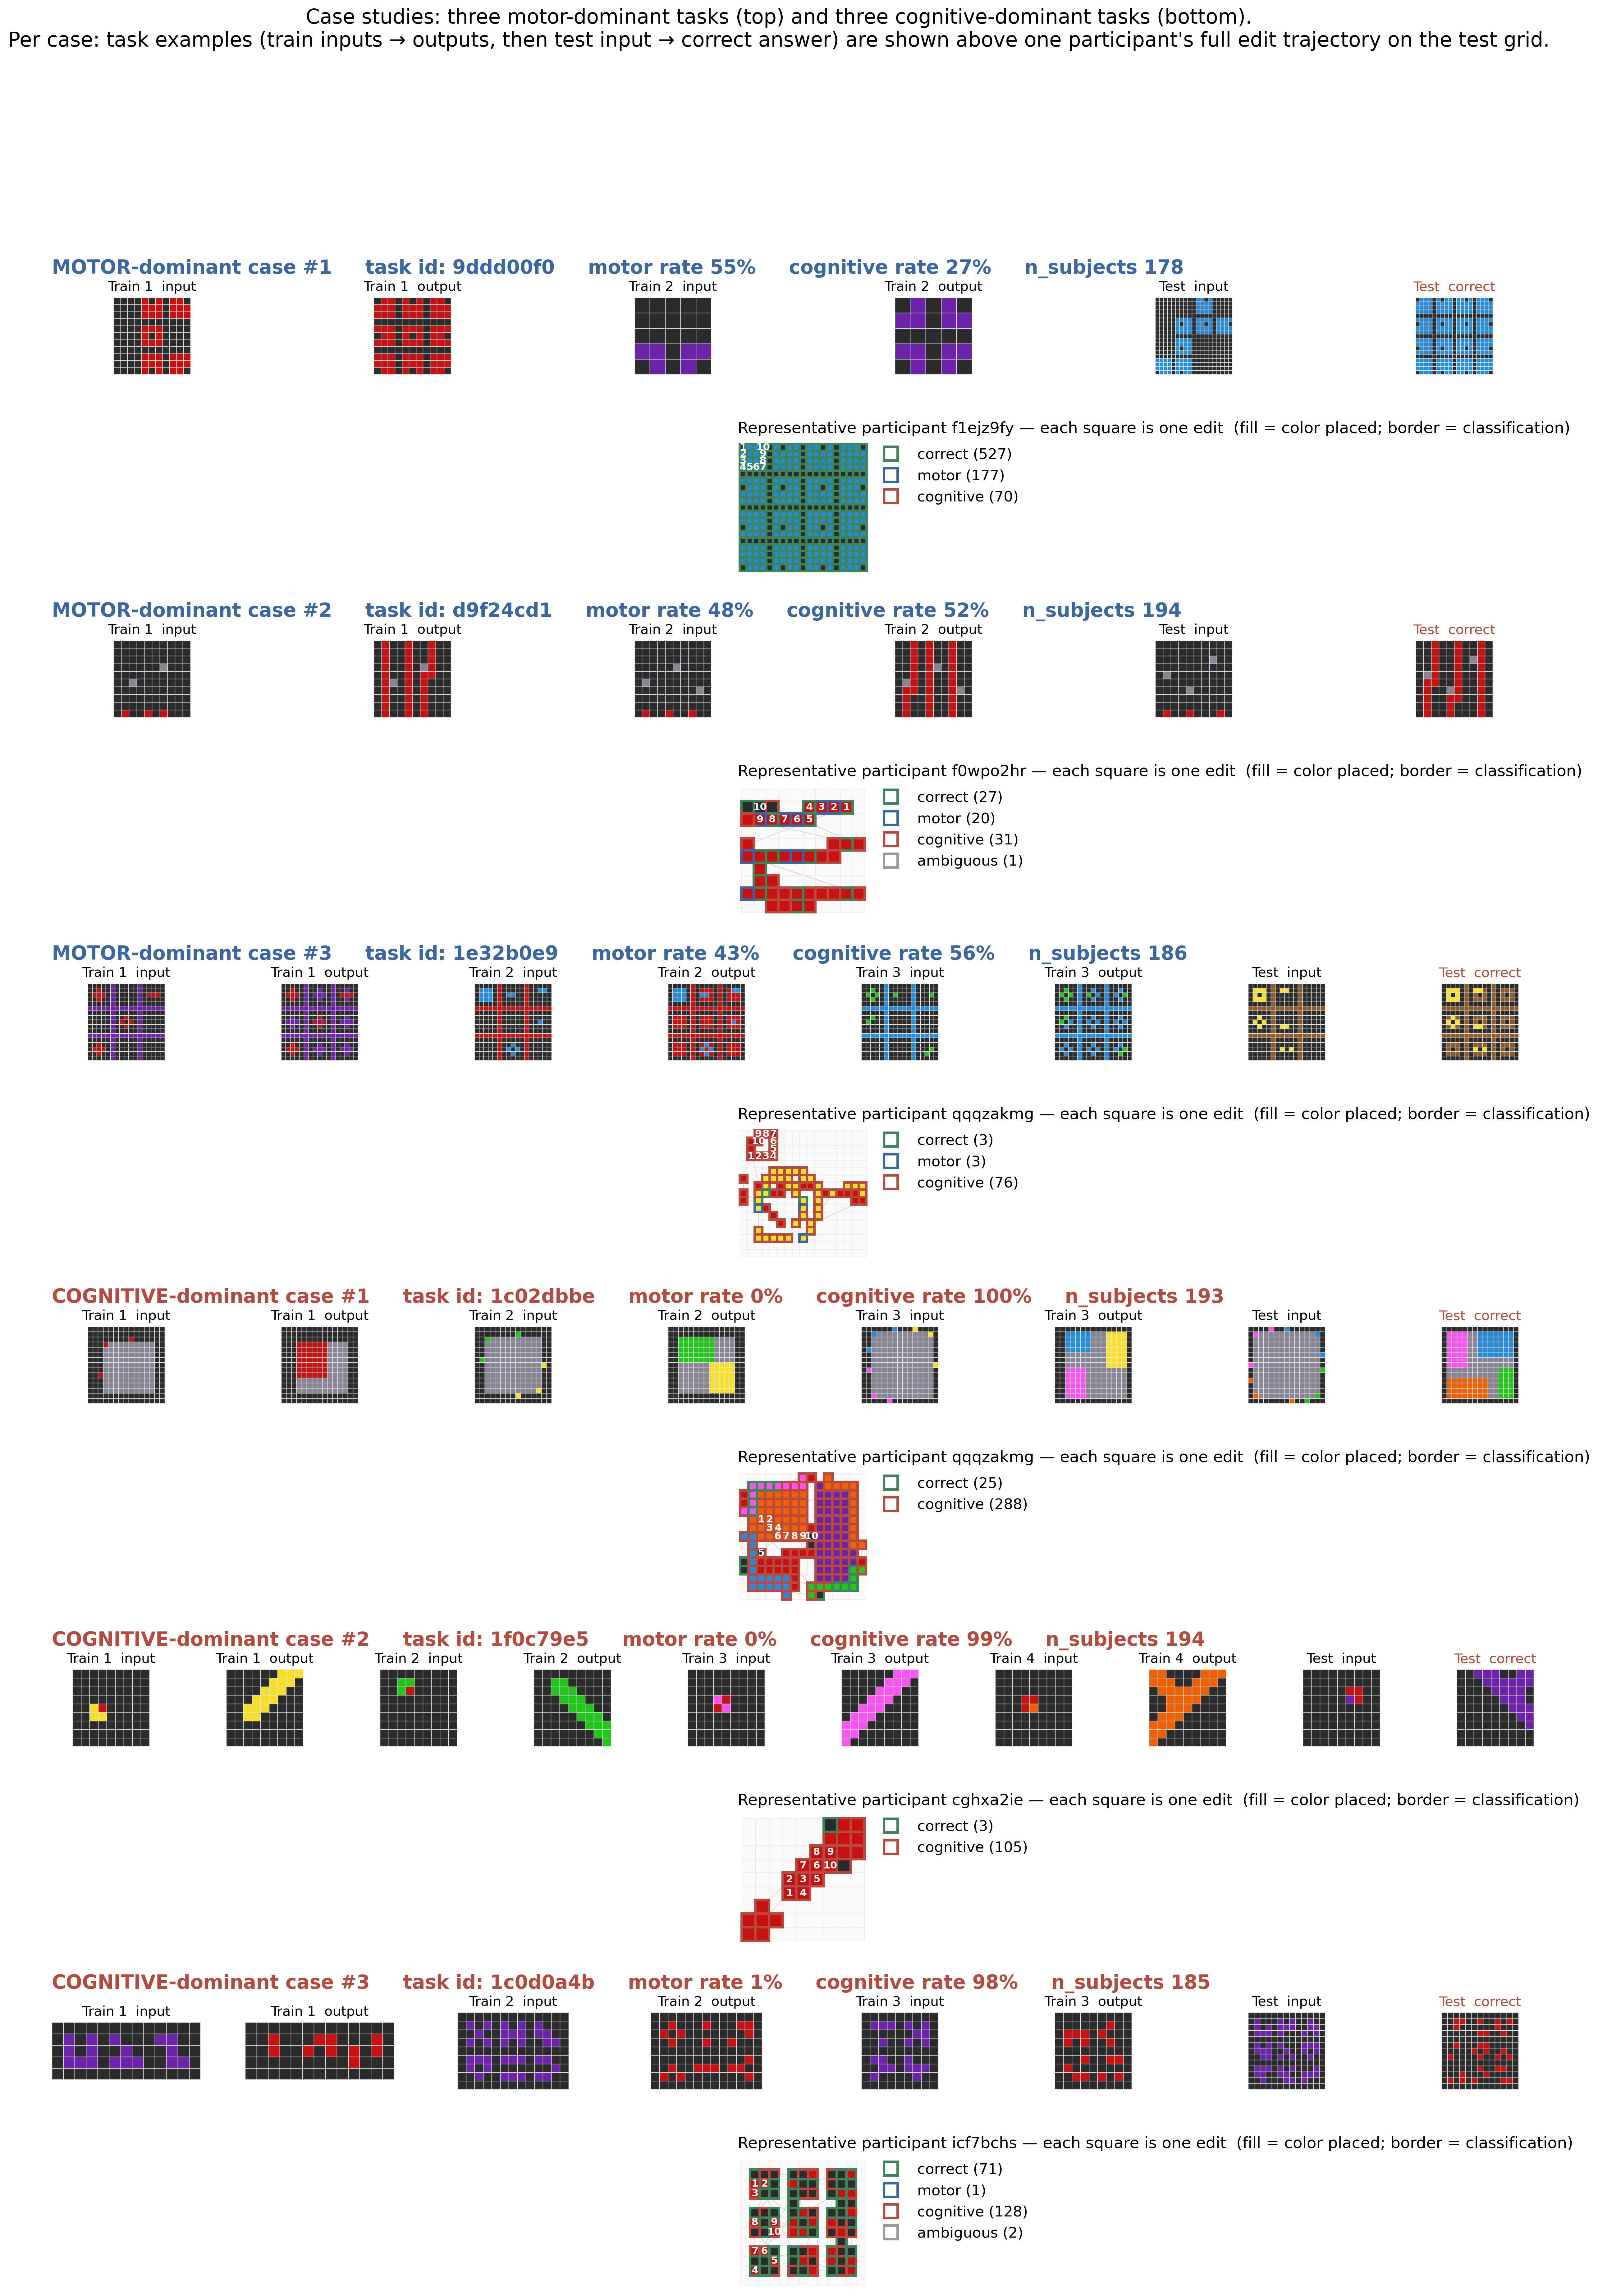
\includegraphics[width=\linewidth]{figures/motor_cognitive_case_studies.png}
  \caption{Six case-study tasks (three motor-dominant, three
  cognitive-dominant) with Success, test input, and a representative
  human trajectory overlayed with per-edit classification. On
  \texttt{9ddd00f0} (top-left, motor-dominant) wrong edits are 1--2
  cells off the correct shape; on \texttt{1f642eb9} (top-right,
  cognitive-dominant) the participant executes a coherent but wrong
  rule spanning the whole grid.}
  \label{fig:motor-case}
\end{figure}


\section{Chunks as self-defined cognitive units}
\label{sec:chunks}

Pause-segmented chunks correspond to the segments between natural
pauses in drawing. They are a participant's own definition of a
cognitive unit: ``draw this one thing, then stop and plan the next.''

\subsection{Per-chunk structure}

Pooled over 40{,}000+ chunks from 75 tasks we observe a clean
feature hierarchy:

\begin{center}
\begin{tabular}{lr}
\toprule
\textbf{Chunk property} & \textbf{Fraction} \\
\midrule
single-color (dominant color $\geq 95\%$ of edits)  & 0.86 \\
one 4-connected component                           & 0.69 \\
multiple CCs but single-color                       & 0.17 \\
row-aligned                                         & 0.37 \\
col-aligned                                         & 0.36 \\
on a single NW--SE or NE--SW diagonal               & 0.06 \\
mean nearest-neighbour chain rate                   & 0.85 \\
\bottomrule
\end{tabular}
\end{center}

Color homogeneity is near-universal, spatial contiguity is common
but not required, and axis alignment is a secondary structural
choice. The 17\% of chunks that span multiple connected components
while staying single-color are the clearest evidence that the
participant's \emph{color} variable sometimes wins over their
\emph{spatial} variable, a pattern we call ``color-over-connectivity.''

\subsection{Drawing strategy example}

Figure \ref{fig:strategy} illustrates the full chunking pipeline on a
single task: first-touch order over Success components, per-chunk
footprint, colour vs shape regimes, and an exemplar trajectory colored
by chunk membership.

\begin{figure}[H]
  \centering
  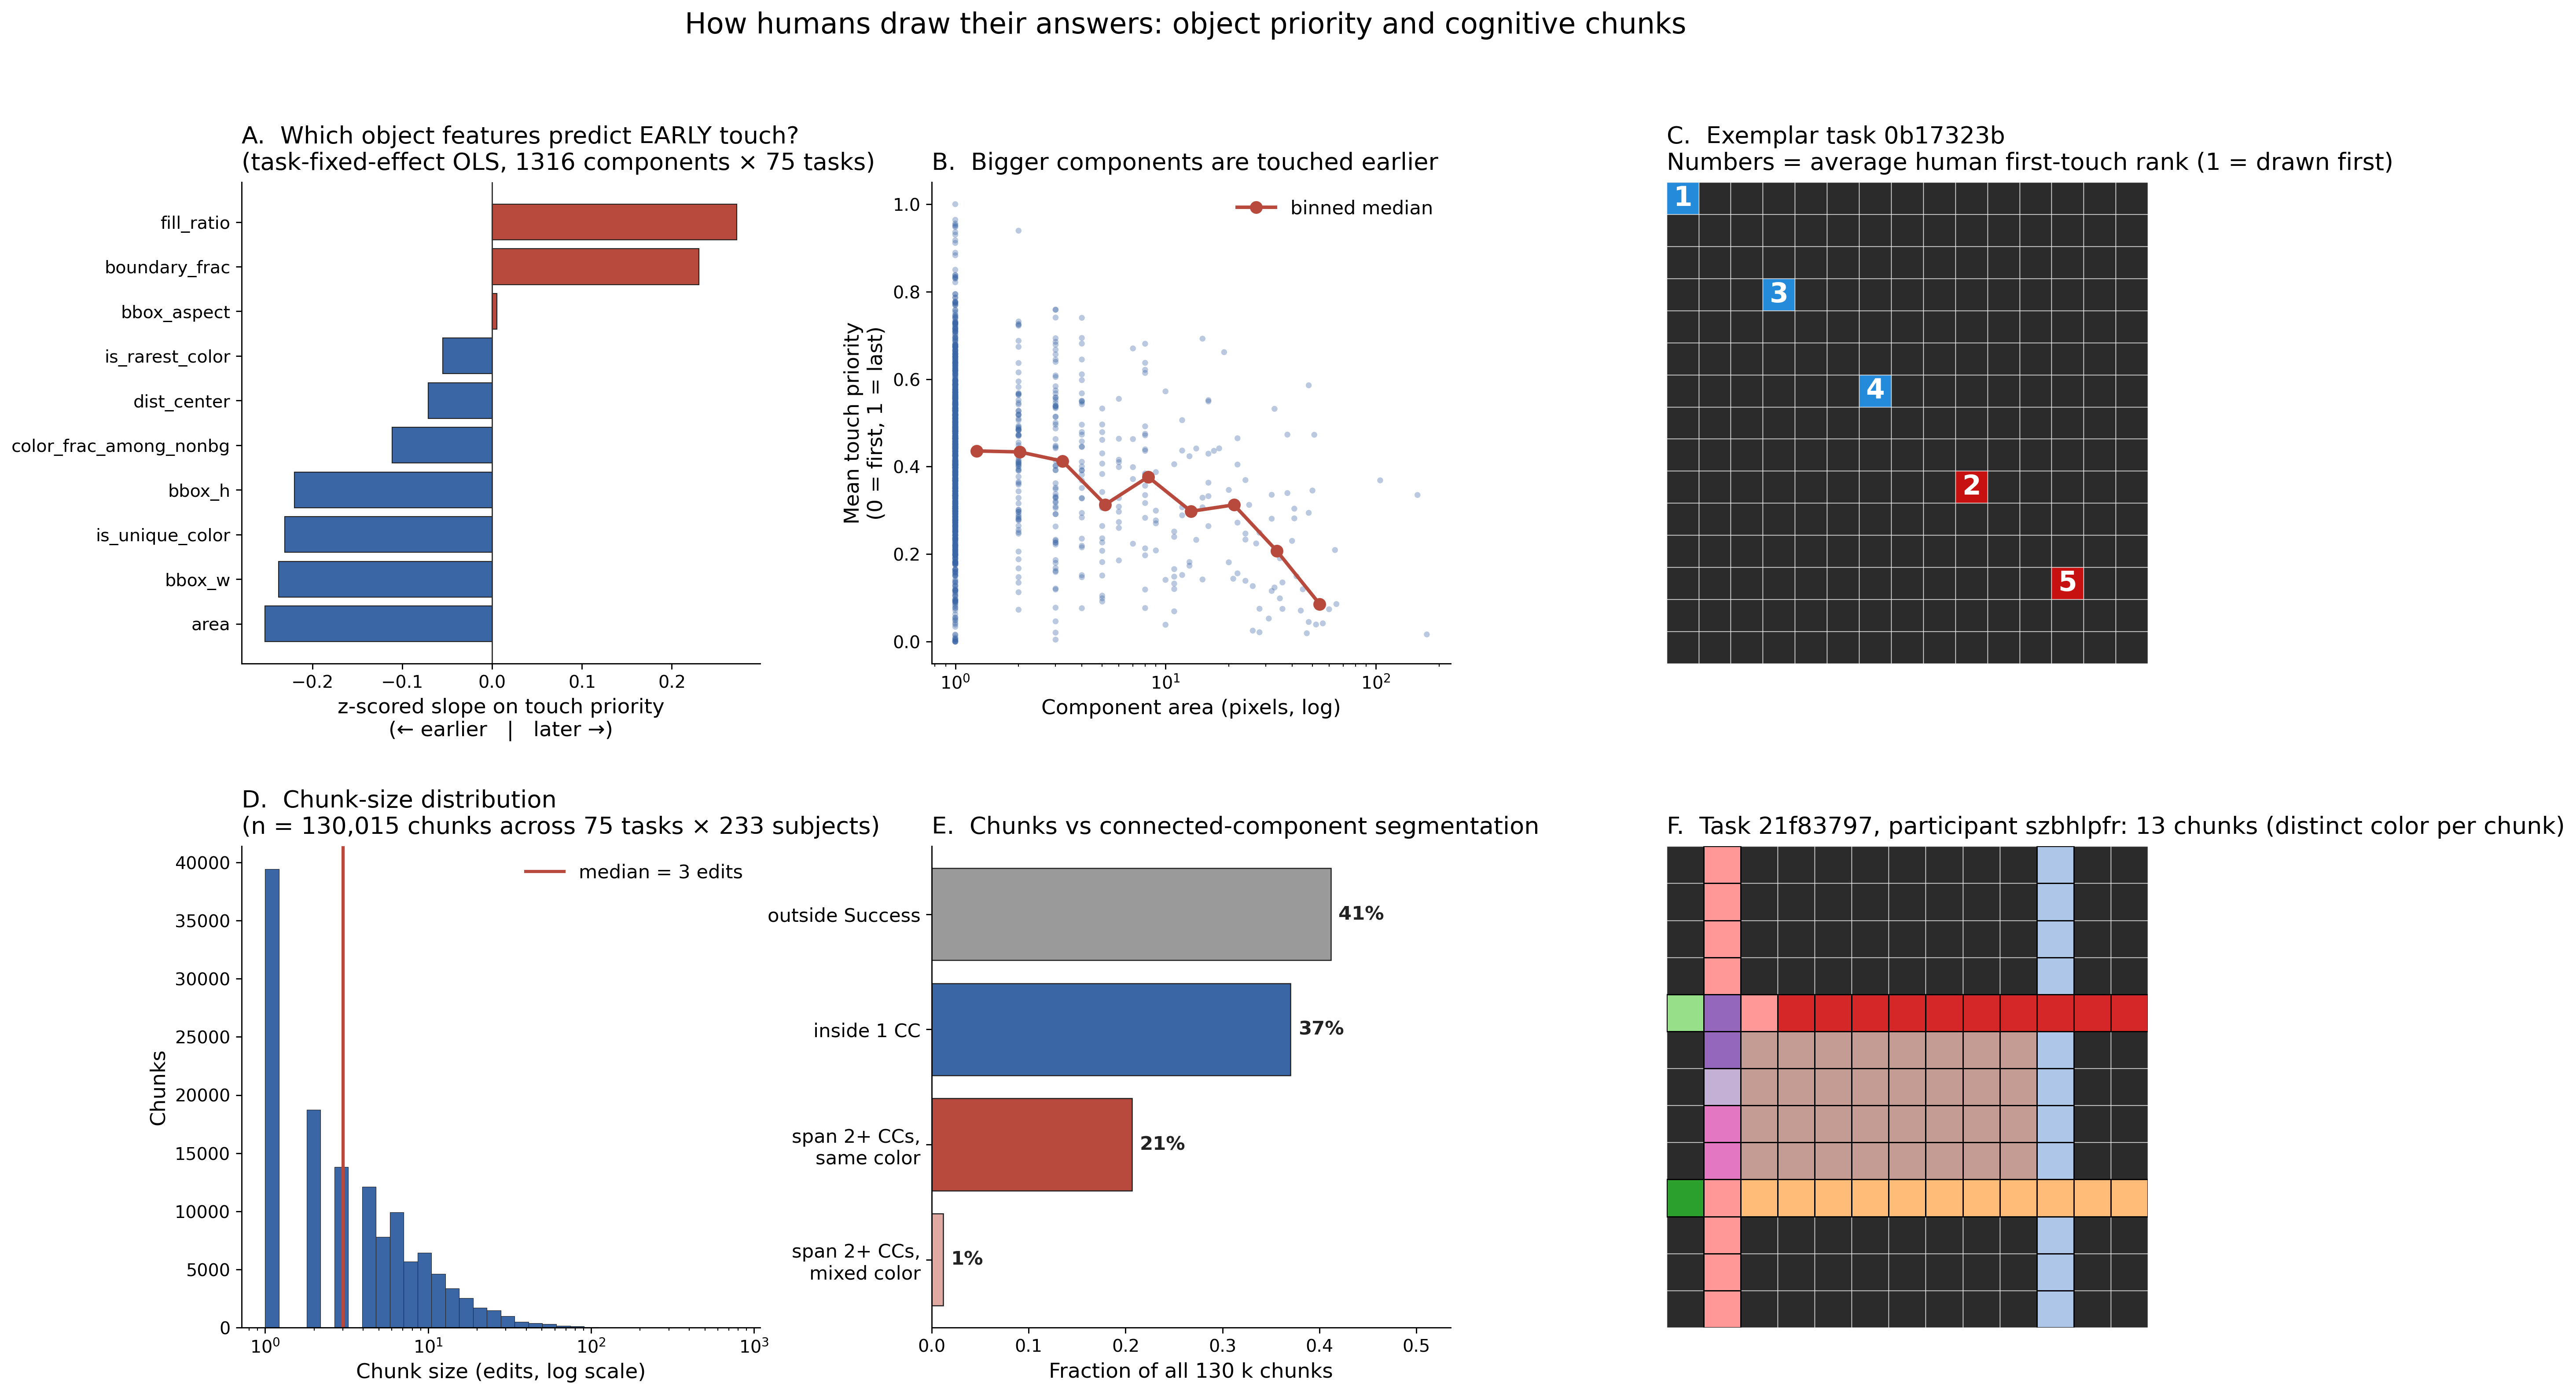
\includegraphics[width=\linewidth]{figures/drawing_strategy_figure.png}
  \caption{Chunking and component priority on representative tasks.
  (A) First-touch rank of Success components by area and
  uniqueness-of-color; (B) per-chunk feature distributions; (C)
  color-vs-connectivity regime for one color-indexed task vs one
  object-indexed task; (D) chunk-size vs IoU scatter; (E) chunk count
  per task against Success-component count; (F) exemplar trajectory
  colored by chunk index.}
  \label{fig:strategy}
\end{figure}

A component-priority regression (OLS with task fixed effects) on
first-touch rank finds that \texttt{area} ($\beta = -0.25$,
$p < 10^{-6}$) and \texttt{is\_unique\_color} ($\beta = -0.23$,
$p < 10^{-5}$) are the two dominant predictors: larger components
and uniquely-colored components are drawn first. Figure
\ref{fig:colorvscc} gives a paired color-vs-CC illustration on two
tasks where the two principles would predict different orderings.

\begin{figure}[H]
  \centering
  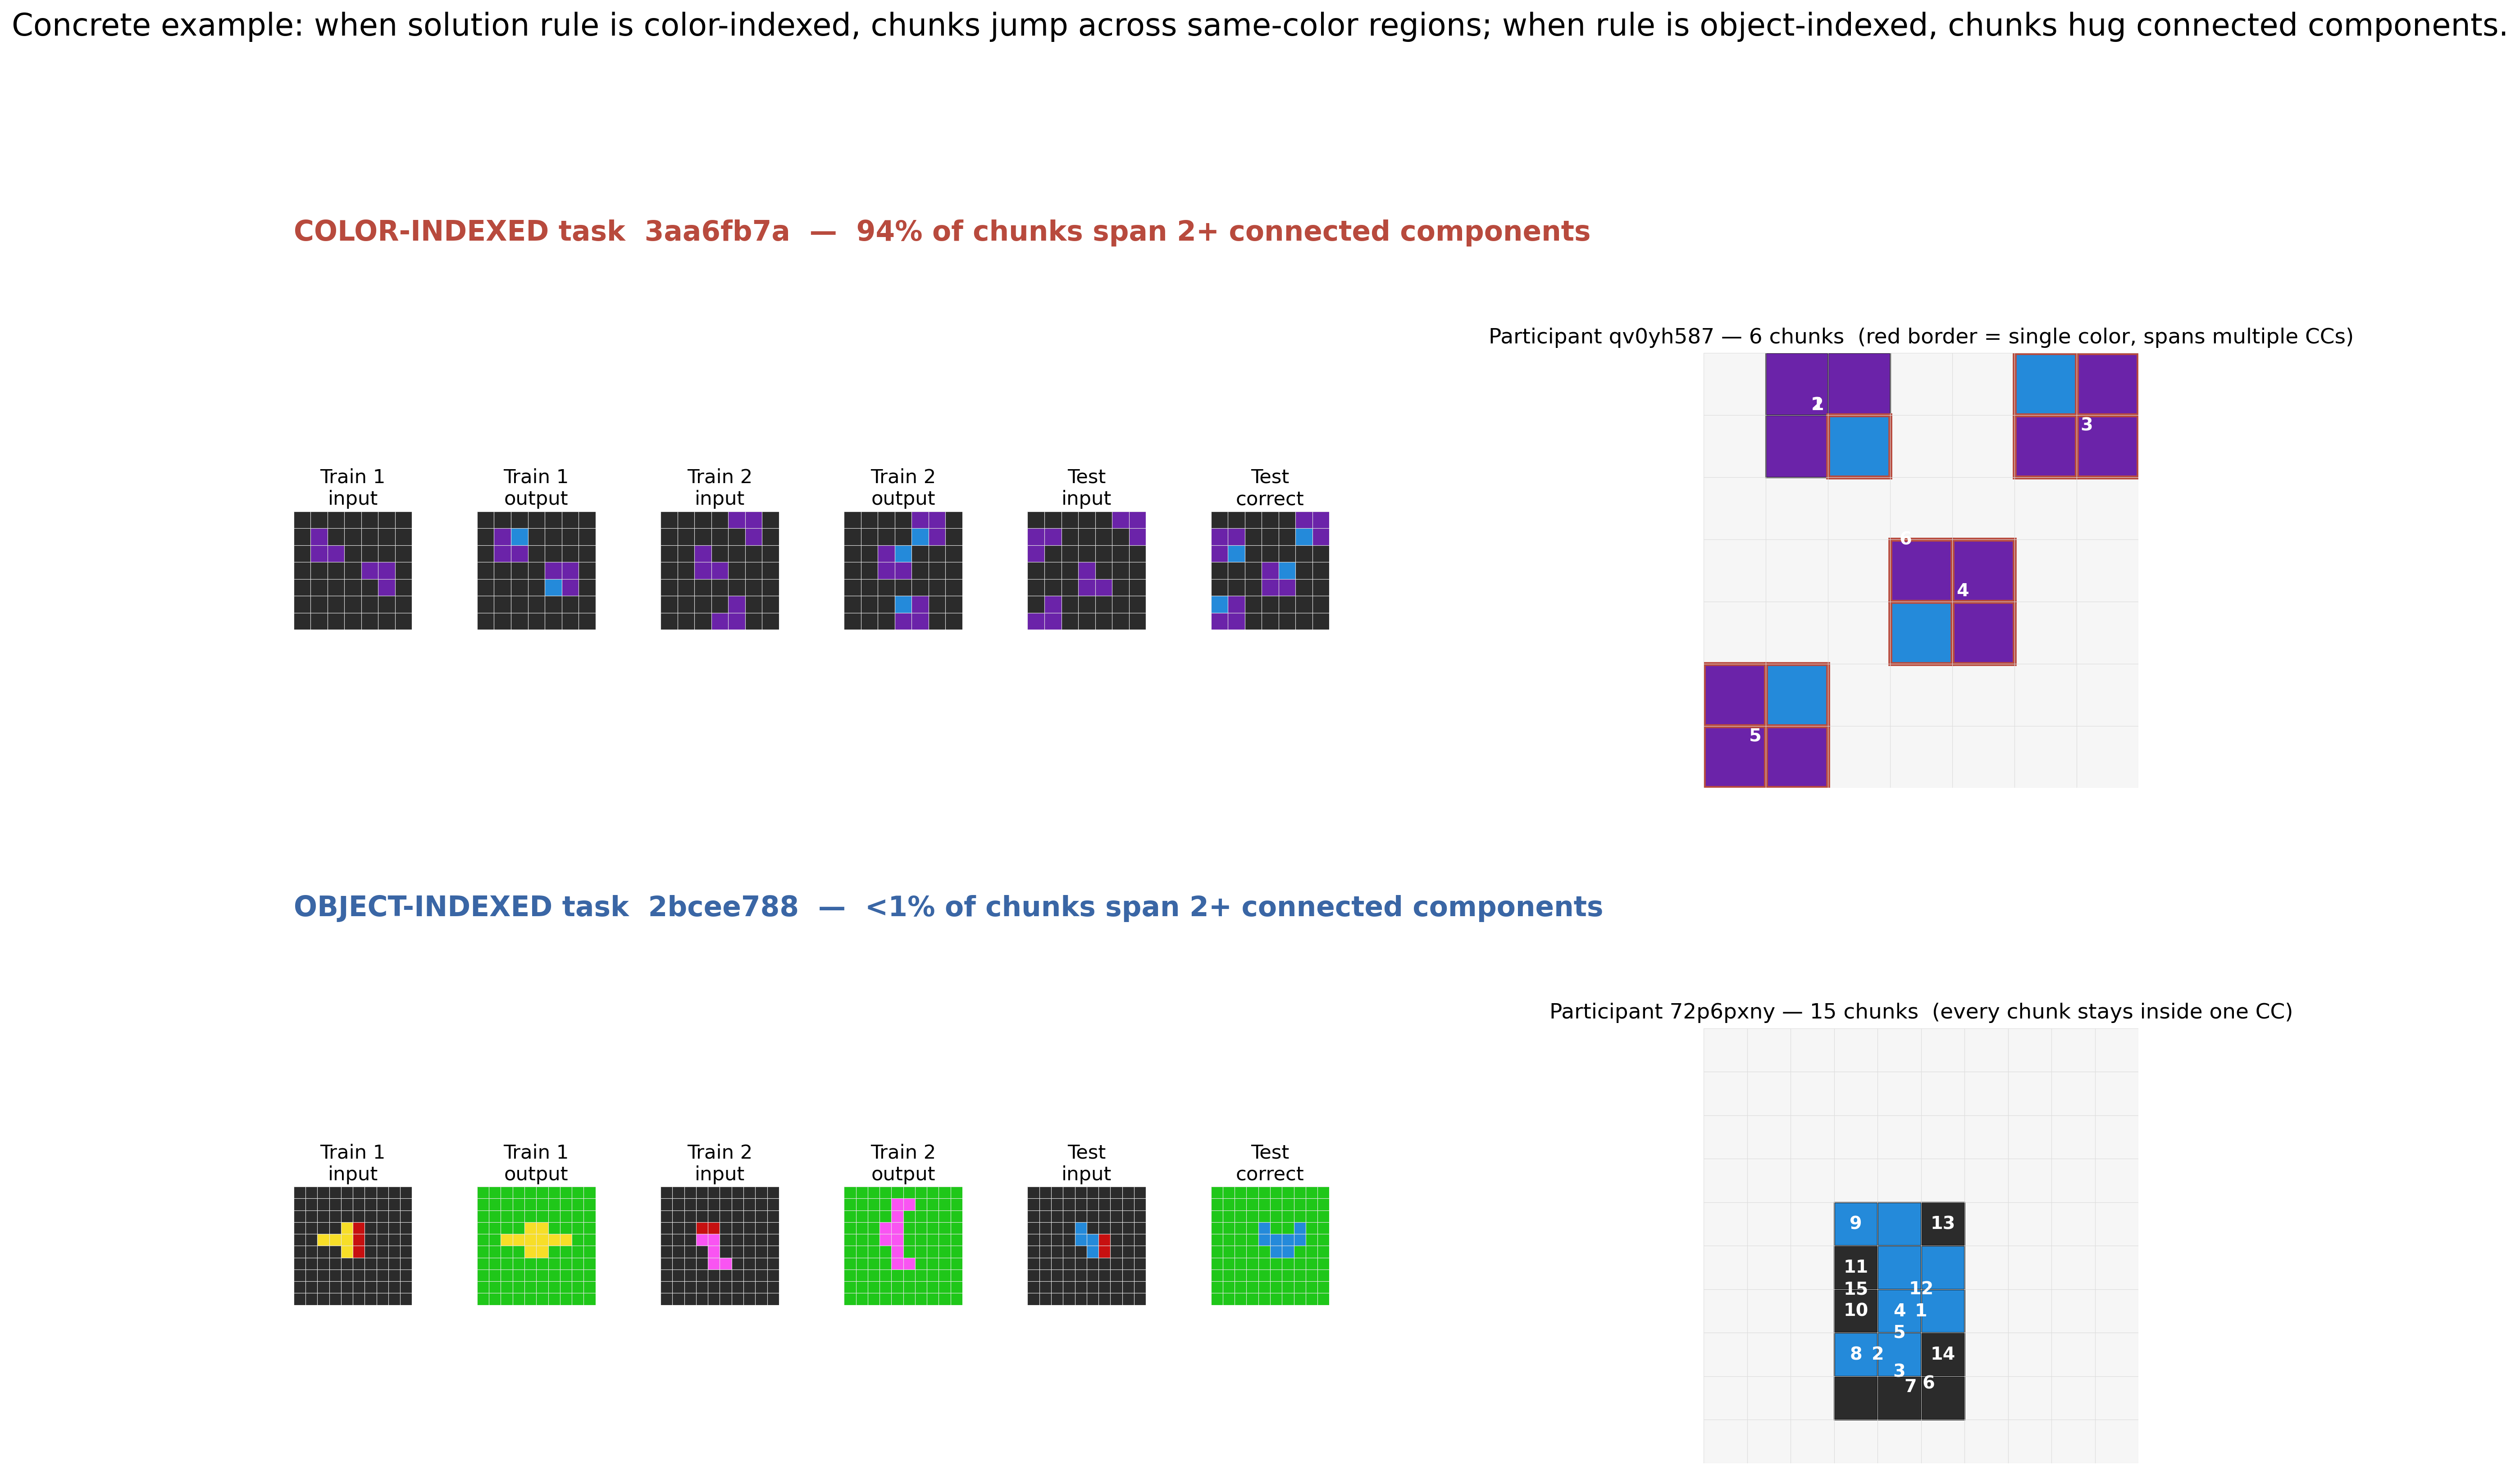
\includegraphics[width=0.9\linewidth]{figures/color_vs_cc_example.png}
  \caption{Color-indexed vs object-indexed tasks. Left: a task whose
  transformation rule keys off color class; chunks align with Success
  color classes regardless of 4-connectivity. Right: a task whose
  rule keys off distinct objects; chunks align with 4-connected
  components. The same participants use different structural
  variables on different tasks.}
  \label{fig:colorvscc}
\end{figure}


\section{Humans vs canonical strategies}
\label{sec:strategies}

\subsection{Six synthetic baselines}

To separate ``humans follow \emph{a} strategy'' from ``the task
forces the strategy'' we defined six canonical synthetic strategies
that each take a Success grid and produce an ordered sequence of
chunks: \texttt{object\_first} (CCs by area), \texttt{color\_first}
(color classes), \texttt{nn\_color\_first} (color class + nearest-
neighbour chaining within a color), \texttt{row\_first},
\texttt{col\_first}, \texttt{random\_k3} (arbitrary groups of 3
cells). Each strategy produces a feature vector identical in shape
to the human chunk fingerprint.

\subsection{No single strategy dominates}

Figure \ref{fig:radar} shows the pooled chunk-feature fingerprint
for humans and each of the six strategies on a radar plot
(panel A), the per-task winner distribution (panel B, $n = 75$
tasks), and two concrete task examples where different strategies
win (panel C). Humans are \emph{not} any single canonical strategy:
on 75 tasks, \texttt{object\_first} wins on 21, \texttt{random\_k3}
on 15, \texttt{row\_first} on 14, \texttt{color\_first} on 10,
\texttt{col\_first} on 8, \texttt{nn\_color\_first} on 7. The
winner depends on the task.

\begin{figure}[H]
  \centering
  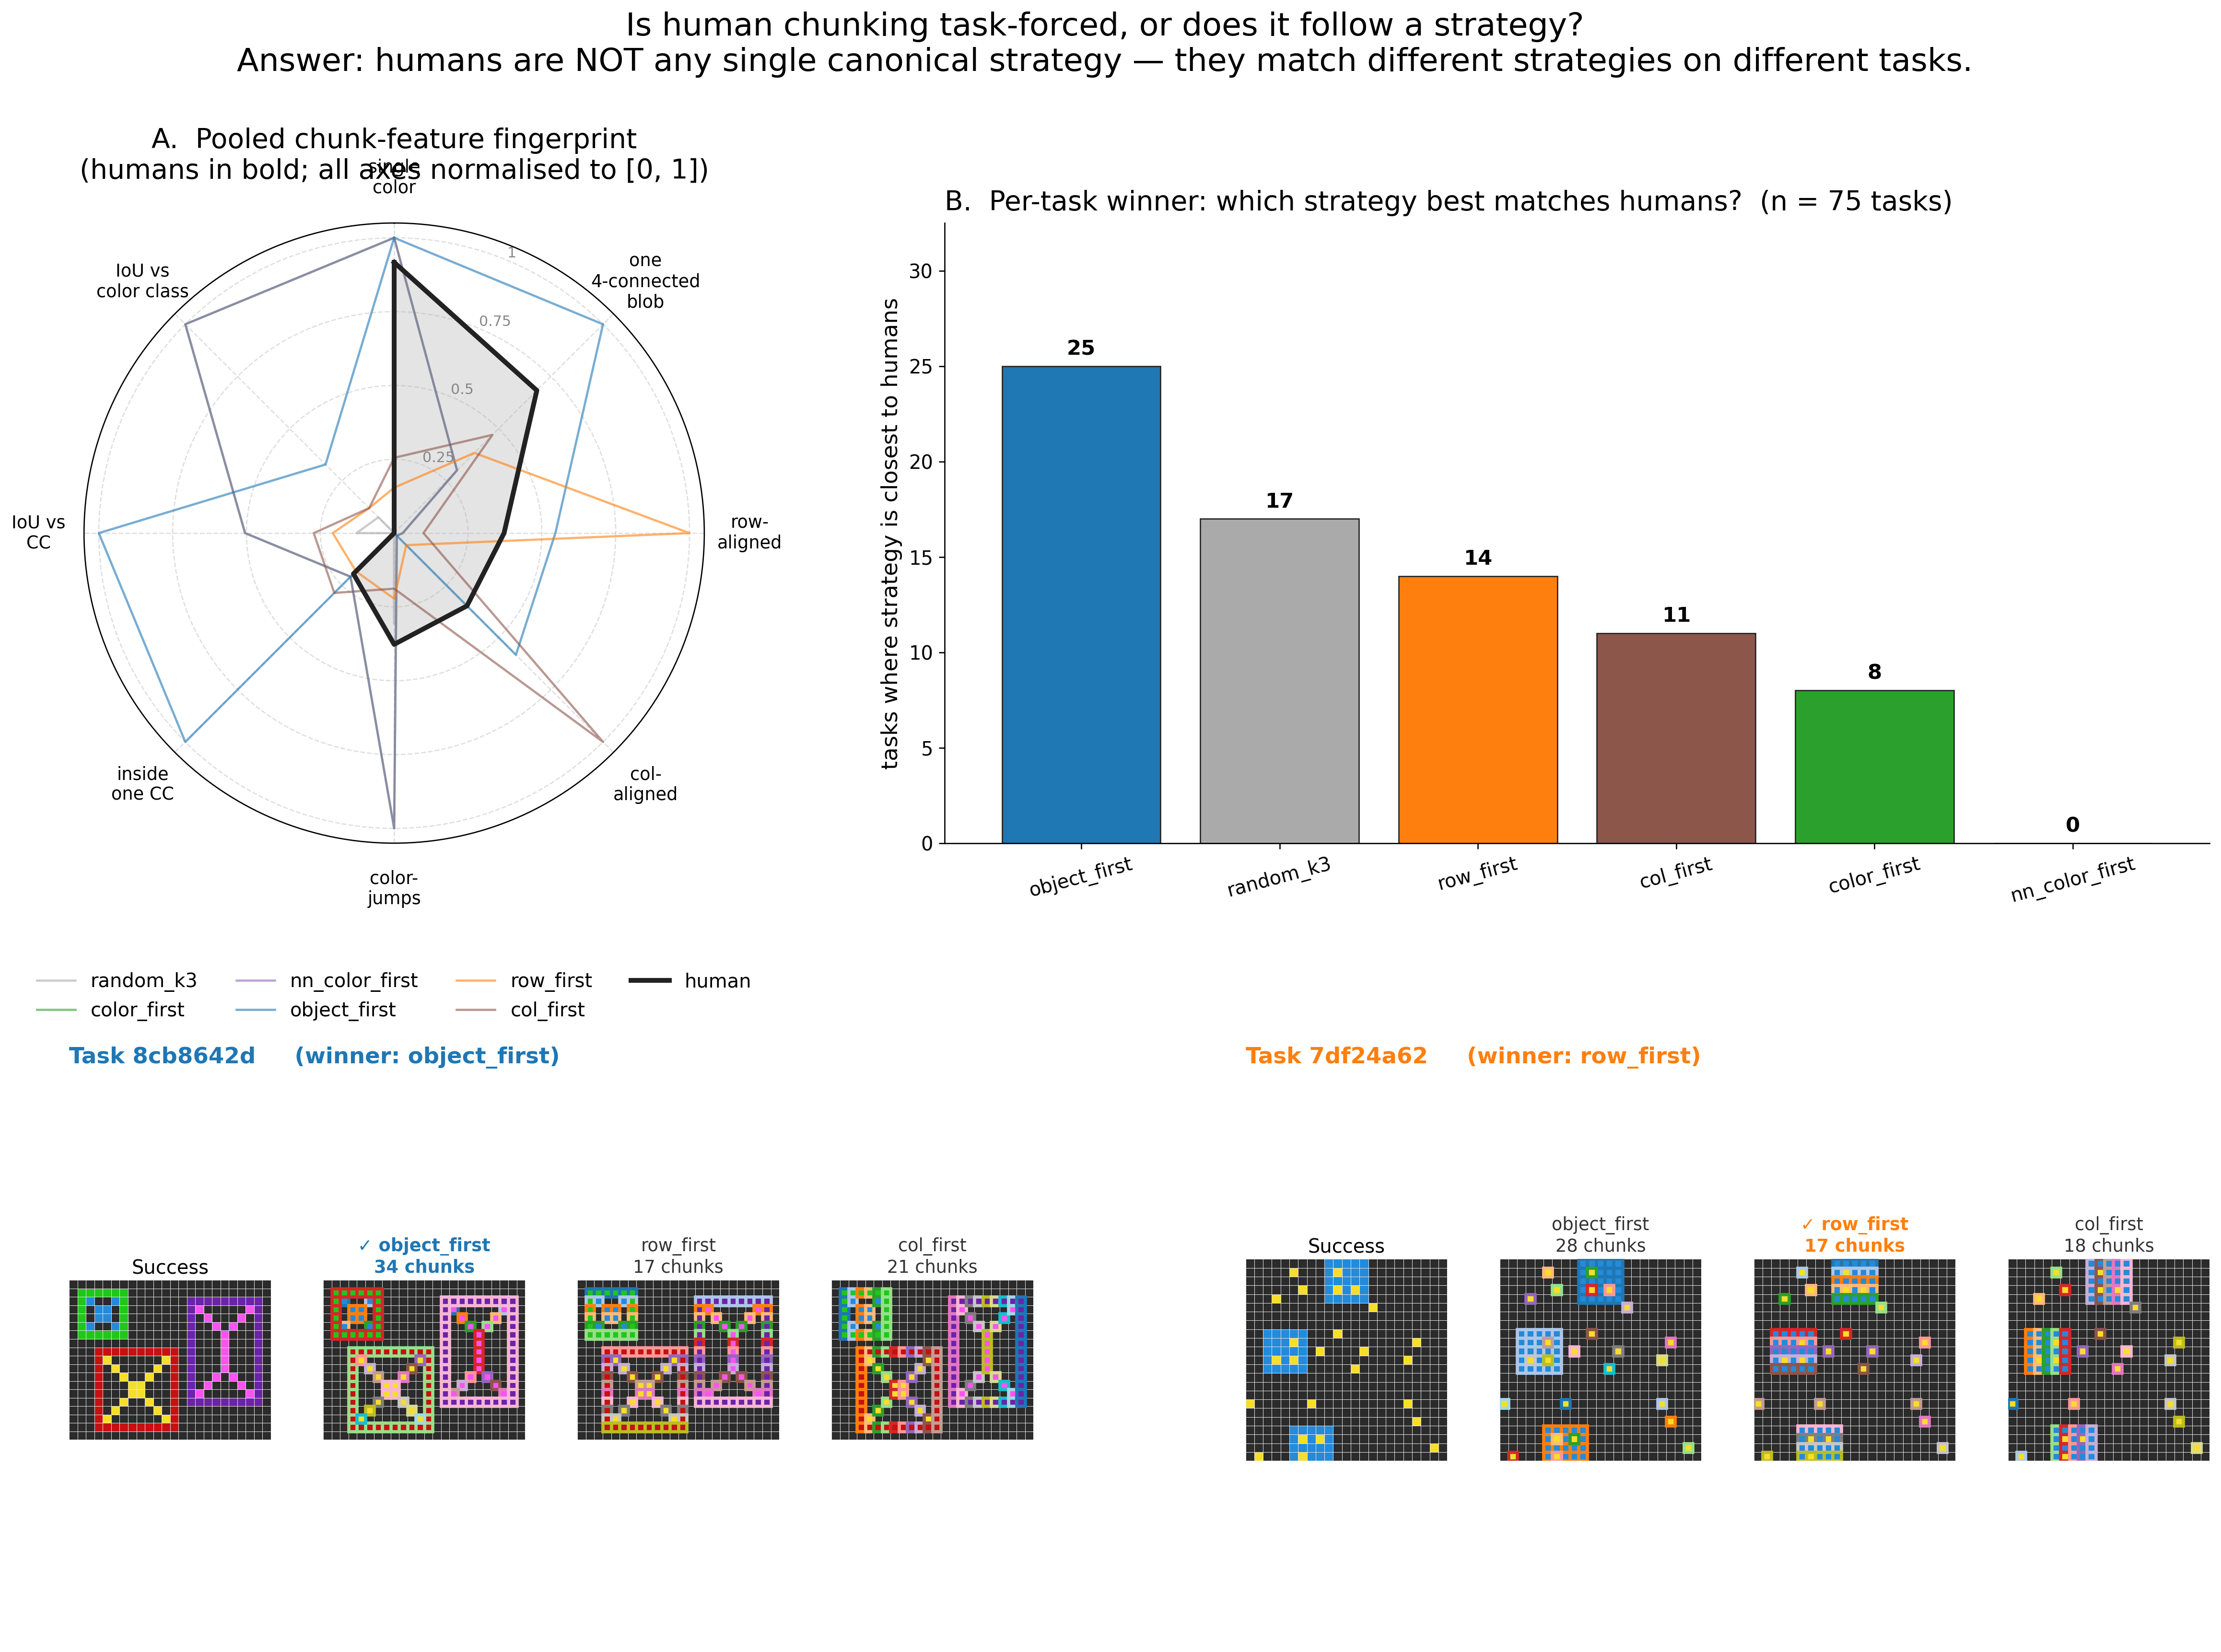
\includegraphics[width=\linewidth]{figures/strategies_vs_human_figure.png}
  \caption{Humans vs six canonical strategies. (A) Pooled chunk-
  feature fingerprint on a radar plot (human in black, strategies in
  color; axes normalised to $[0,1]$). (B) Per-task winner: which
  synthetic strategy's fingerprint is closest to humans; 75 tasks.
  (C) Two concrete task examples where different strategies win,
  with Success grids and candidate chunk overlays.}
  \label{fig:radar}
\end{figure}


\section{What about the task forces strategy choice?}
\label{sec:taskpredictors}

\subsection{Affordance is nearly constant}

For each task $\times$ strategy pair we defined \emph{affordance}
$= (\text{strategy produces} \geq 2\ \text{chunks})$. Counting
afforded strategies per task: 67 of 75 tasks afford \emph{all six}
canonical strategies. The 8 constrained tasks are all single-output-
color tasks that disable \texttt{color\_first}/
\texttt{nn\_color\_first}. Affordance alone cannot explain which
strategy humans pick.

\subsection{Per-strategy usage is predicted by task features}

Using \emph{subject-level} closest-strategy assignment we compute
per-task usage shares for each canonical strategy and correlate them
against 14 task-intrinsic features (grid dimensions, cell counts,
color counts, connected-component statistics, symmetry scores) plus
four interface-shortcut rates from Experiment-2
(\texttt{used\_copy\_mean}, \texttt{n\_showex\_mean},
\texttt{n\_reset\_mean}, \texttt{n\_edits\_mean}). Table
\ref{tab:taskpred} lists the strongest predictors.

\begin{table}[H]
\small
\centering
\caption{Strongest predictors of per-task subject-usage share
for each canonical strategy. Spearman correlations, $n = 75$ tasks.
Entries with $|\rho| \geq 0.25$ and $p < 0.05$ shown.}
\label{tab:taskpred}
\begin{tabular}{llrr}
\toprule
\textbf{Strategy} & \textbf{Predictor} & \textbf{Spearman $\rho$} &
  \textbf{$p$} \\
\midrule
object\_first & n\_success\_cc          & $+0.39$ & $0.001$ \\
color\_first  & n\_colors\_output       & $+0.48$ & $<10^{-3}$ \\
color\_first  & n\_new\_colors          & $+0.25$ & $0.028$ \\
col\_first    & n\_reset\_mean          & $+0.34$ & $0.003$ \\
col\_first    & symmetry\_h             & $+0.30$ & $0.010$ \\
row\_first    & n\_success\_cc          & $-0.27$ & $0.021$ \\
random\_k3    & mean\_cc\_area          & $-0.58$ & $<10^{-3}$ \\
random\_k3    & max\_cc\_area           & $-0.47$ & $<10^{-3}$ \\
random\_k3    & n\_cells\_nonbg         & $-0.31$ & $0.007$ \\
\bottomrule
\end{tabular}
\end{table}

Reading: more distinct connected components $\Rightarrow$ more
subjects draw object-by-object; more output colors $\Rightarrow$
more subjects sort by color; small outputs (few cells, tiny objects)
produce chunks whose fingerprint resembles the \texttt{random\_k3}
baseline (best interpreted as ``no canonical strategy dominates'').
Horizontal symmetry and higher \texttt{n\_reset\_mean} favour
column-first; interface shortcuts other than reset (copy, show-
example) barely shift strategy choice.

Figure \ref{fig:task-strategy} combines these results into a single
display: affordance histogram (A), dominant-strategy fraction
distribution (B, mean $= 0.68$), the full task-feature $\times$
strategy-usage heatmap (C), three scatter plots of the strongest
predictors (D), and two concrete examples of a low-entropy and a
high-entropy task (E).

\begin{figure}[H]
  \centering
  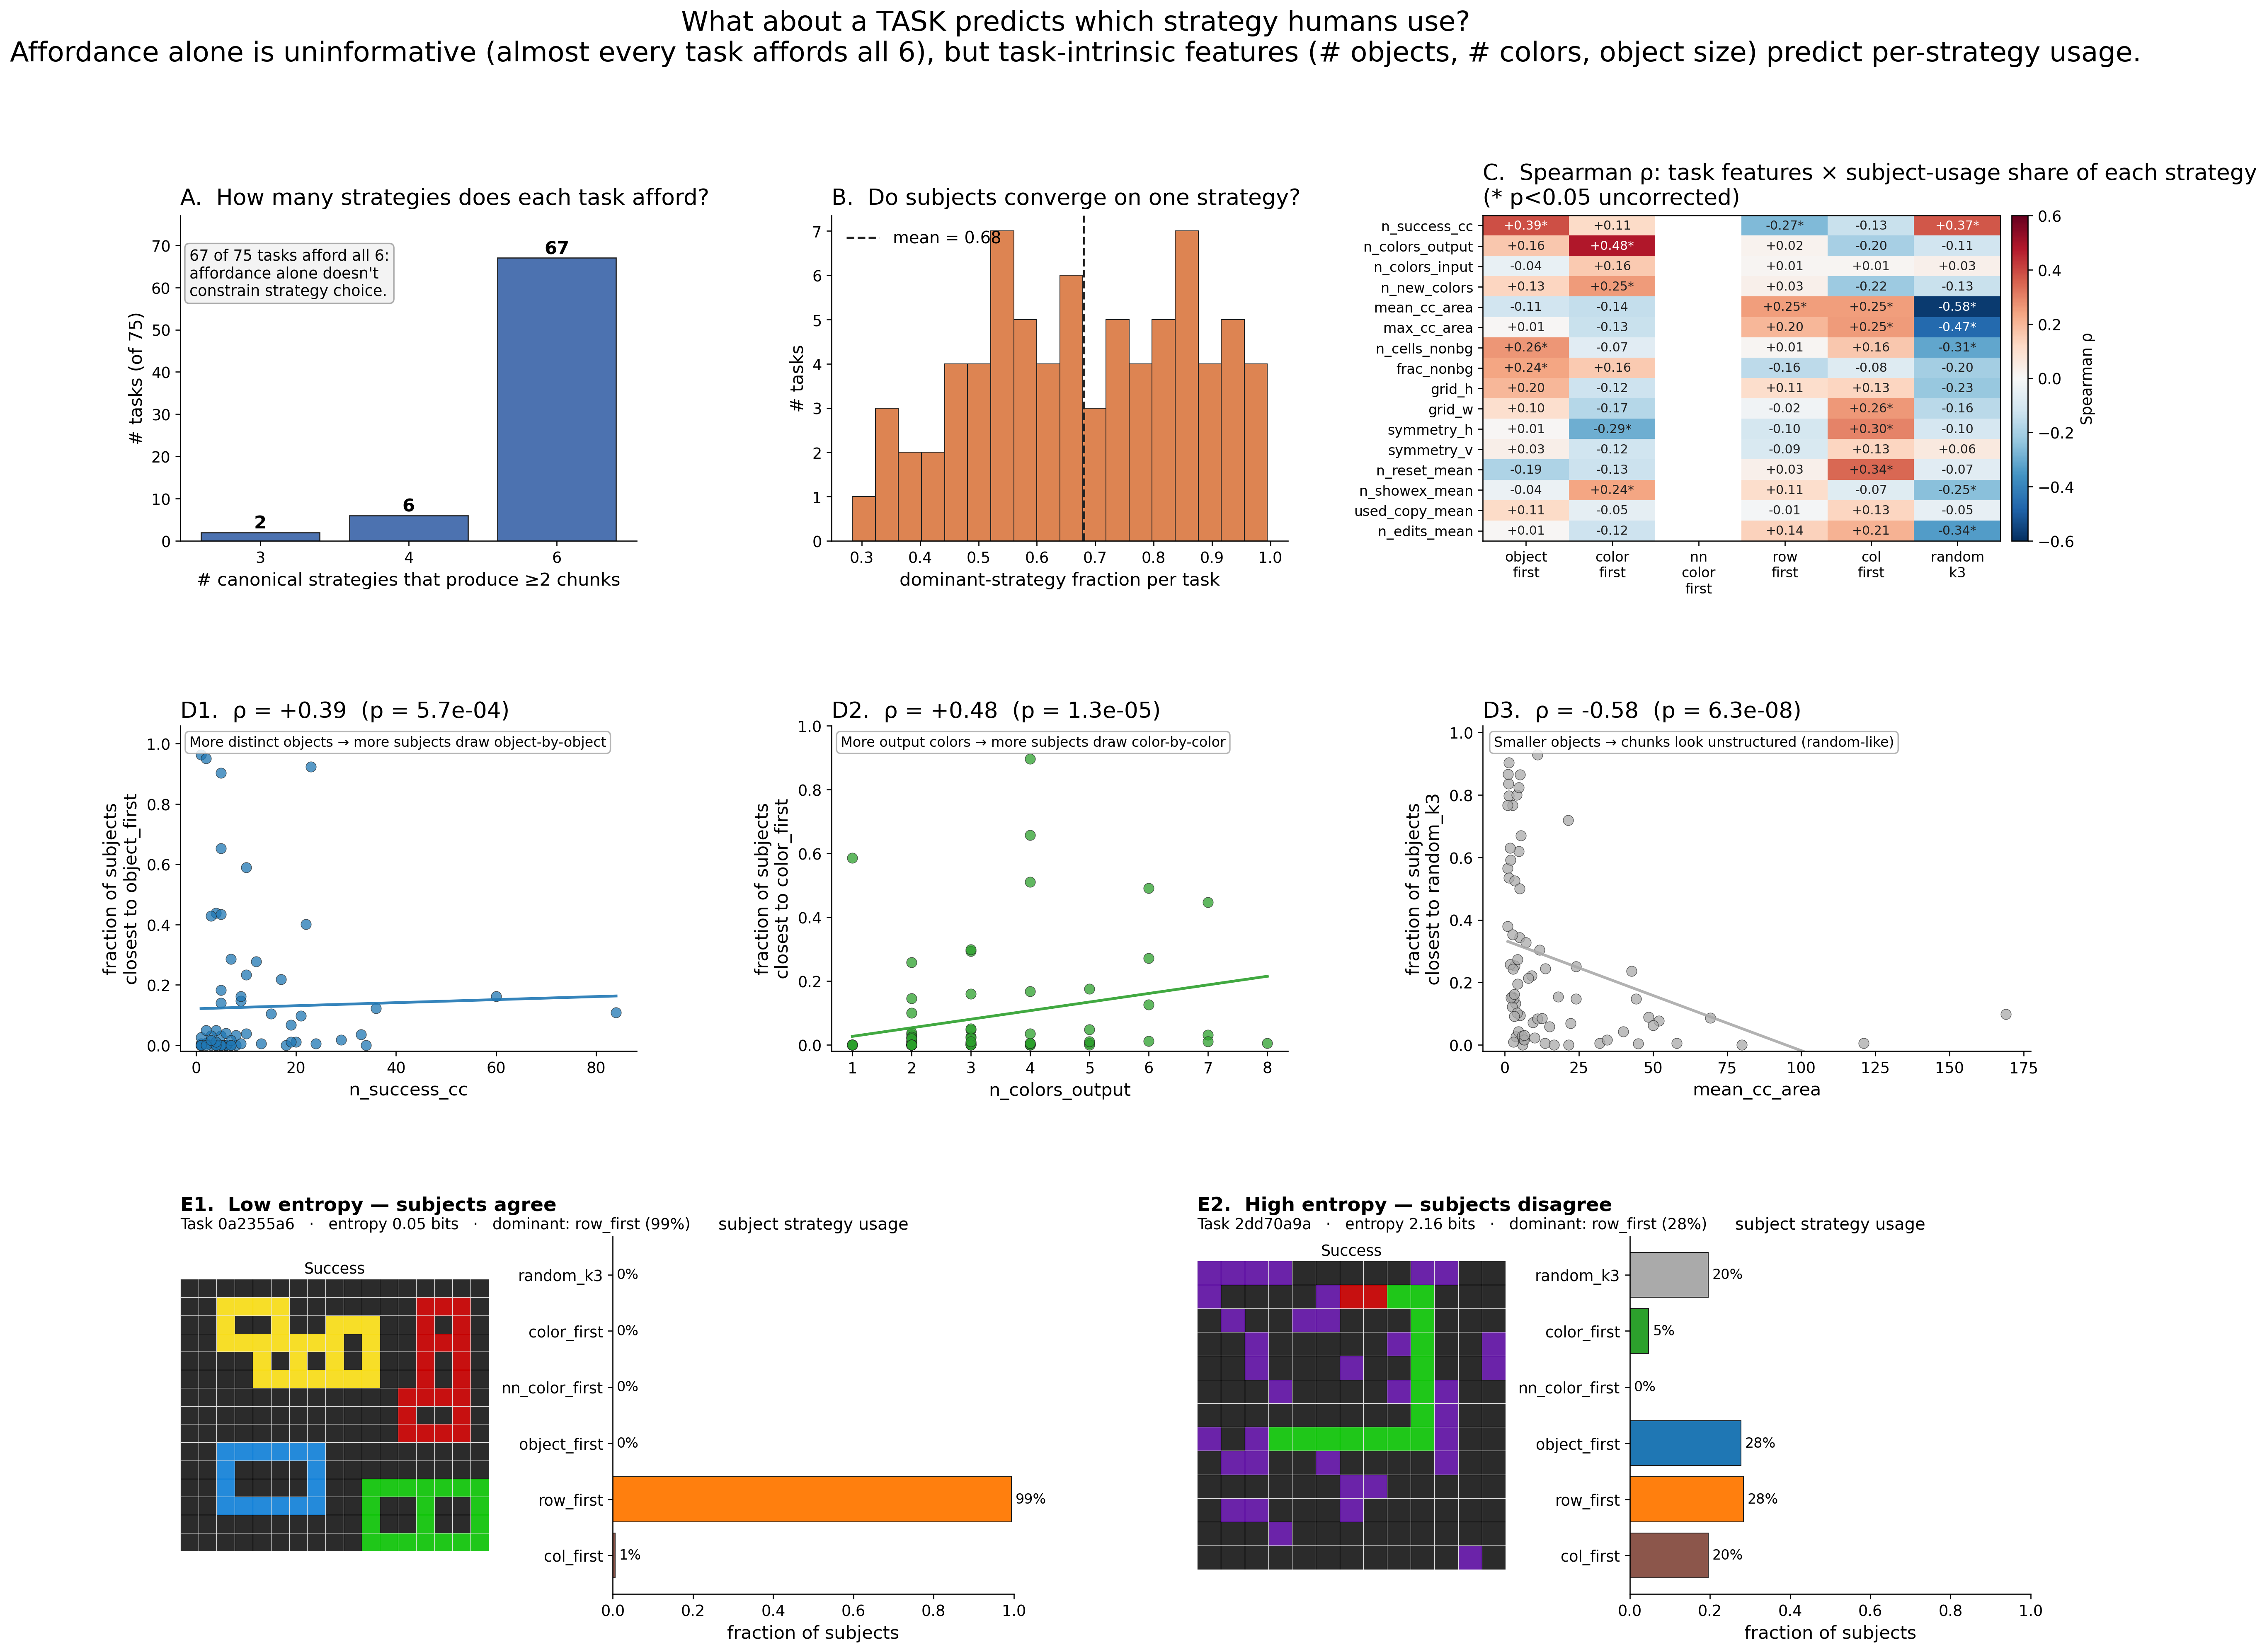
\includegraphics[width=\linewidth]{figures/task_vs_strategy_figure.png}
  \caption{What about the task predicts which strategy humans use?
  (A) Affordance histogram --- 67 of 75 tasks afford all 6 strategies.
  (B) Distribution of the dominant-strategy fraction per task.
  (C) Heatmap of Spearman $\rho$ between task features (rows) and
  per-strategy subject-usage share (columns); $^{*}p<0.05$.
  (D) Three scatter plots of the strongest predictors. (E) Concrete
  task examples: \texttt{0a2355a6} with 99\% row-first subjects,
  \texttt{2dd70a9a} with near-uniform strategy spread.}
  \label{fig:task-strategy}
\end{figure}


\section{Can chunks predict which common error?}
\label{sec:errors}

Given that cognitive errors are systematic wrong plans, we ask
whether a trajectory's chunks carry a signal about \emph{which}
Top Error (TE) the participant will commit. We test four
increasingly-specific voting schemes and condition on task
diagnosability, class balance, and temporal position.

\subsection{Voting schemes}

For each trajectory:

\begin{enumerate}[leftmargin=*, topsep=2pt, itemsep=1pt]
  \item \textbf{Raw IoU vote} --- each chunk votes for the label
        (Success, TE1, TE2, \ldots) whose 4-connected components
        give it the highest IoU.
  \item \textbf{Diagnostic-cells vote} --- each label's
        \emph{diagnostic mask} is the set of cells where that
        label's color is \emph{unique} compared to every other
        label. Chunks vote using overlap with diagnostic masks.
  \item \textbf{Color-aware diagnostic vote} --- each label's
        diagnostic set consists of $(y, x, \text{color})$
        \emph{triples}: the chunk matches a label only when the
        participant painted \emph{that label's color} at a
        distinguishing cell. Votes are weighted by match counts.
  \item \textbf{Temporal subsets} --- compute the color-aware
        weighted vote using only chunks from the first quarter,
        first half, or last half of the trajectory.
\end{enumerate}

Ground truth for each trajectory is the label of its submitted
grid.

\subsection{Raw vote inflates, diagnostic cells are needed}

Raw IoU overall accuracy is 68.1\% against a $\sim$25\% chance
baseline, but this is driven entirely by Success trajectories
(77.8\% correct). On error-ending trajectories, raw IoU collapses
to 17.6\% (TE1), 7.1\% (TE2), 11.5\% (TE3) --- chunks mostly match
Success components even when the participant ends on a wrong
answer, because parts of the wrong answer still overlap with Success.
Restricting to diagnostic masks raises strict-cognitive accuracy
from 17.5\% to 28.3\%.

\subsection{Class imbalance is the ceiling}

On error-ending trajectories TE1 is $\sim$60\% of the data. The
``always predict TE1'' majority baseline beats every voting scheme
on the TE1-vs-TE2 and TE1-vs-TE3 pairs. Table \ref{tab:pairwise}
gives the pairwise picture.

\begin{table}[H]
\small
\centering
\caption{Pairwise discrimination among error-ending trajectories.
Color-aware vote restricted to votes $\in \{\text{TE}_a, \text{TE}_b\}$.
The only pair where chunk prediction beats majority baseline is
TE2 vs TE3, whose class balance is nearly even.}
\label{tab:pairwise}
\begin{tabular}{lrrrr}
\toprule
\textbf{Pair} & \textbf{$n$} & \textbf{chunk acc} &
  \textbf{majority baseline} & \textbf{above baseline} \\
\midrule
TE1 vs TE2   & 491 & 0.705 & 0.721 & $-1.6$ pp \\
TE1 vs TE3   & 402 & 0.808 & 0.841 & $-3.2$ pp \\
\textbf{TE2 vs TE3} & 163 & $\mathbf{0.632}$ & 0.558 & $\mathbf{+7.4\ \text{pp}}$ \\
\bottomrule
\end{tabular}
\end{table}

\subsection{Early chunks predict better than late chunks}

On the balanced pair (TE2 vs TE3, diagnostic-triple pool $\geq 40$):

\begin{center}
\begin{tabular}{lrrr}
\toprule
\textbf{Chunk window} & \textbf{$n$} & \textbf{accuracy} &
  \textbf{baseline} \\
\midrule
first quarter        & 27 & $\mathbf{0.741}$ & 0.556 \\
first half           & 33 & 0.697 & 0.515 \\
all chunks           & 42 & 0.643 & 0.500 \\
last half            & 29 & 0.483 & 0.517 \\
\bottomrule
\end{tabular}
\end{center}

Early chunks beat late chunks by 25.8 percentage points. The wrong
plan is visible at the \emph{start} of the trajectory; late chunks
add noise from fixing, redoing and second-guessing. This is a usable
online signal for a solver that sees partial drawings.

\subsection{Error-prone is a trait; which error is not}

Across 226 subjects with $\geq 5$ trials, split-half Spearman
reliability (50 random splits) is $\rho = +0.35$ for
\texttt{error\_rate} but near zero for each specific TE
(\texttt{te1\_rate} $= +0.11$, \texttt{te2\_rate} $= +0.05$,
\texttt{te3\_rate} $= +0.16$). One-way variance decomposition
($\eta^2$) of trial outcomes by task identity vs subject identity:

\begin{center}
\begin{tabular}{lrr}
\toprule
\textbf{Outcome} & \textbf{$\eta^2$ by task} &
  \textbf{$\eta^2$ by subject} \\
\midrule
any error  & 0.196 & 0.048 \\
TE1        & 0.159 & 0.030 \\
TE2        & 0.052 & 0.031 \\
TE3        & 0.015 & 0.035 \\
\bottomrule
\end{tabular}
\end{center}

Task identity explains 4--5$\times$ more of each outcome than
subject identity. The error signature is \emph{population-level per
task}, not personal.

Figure \ref{fig:chunks-errors} summarises these findings in five
panels.

\begin{figure}[H]
  \centering
  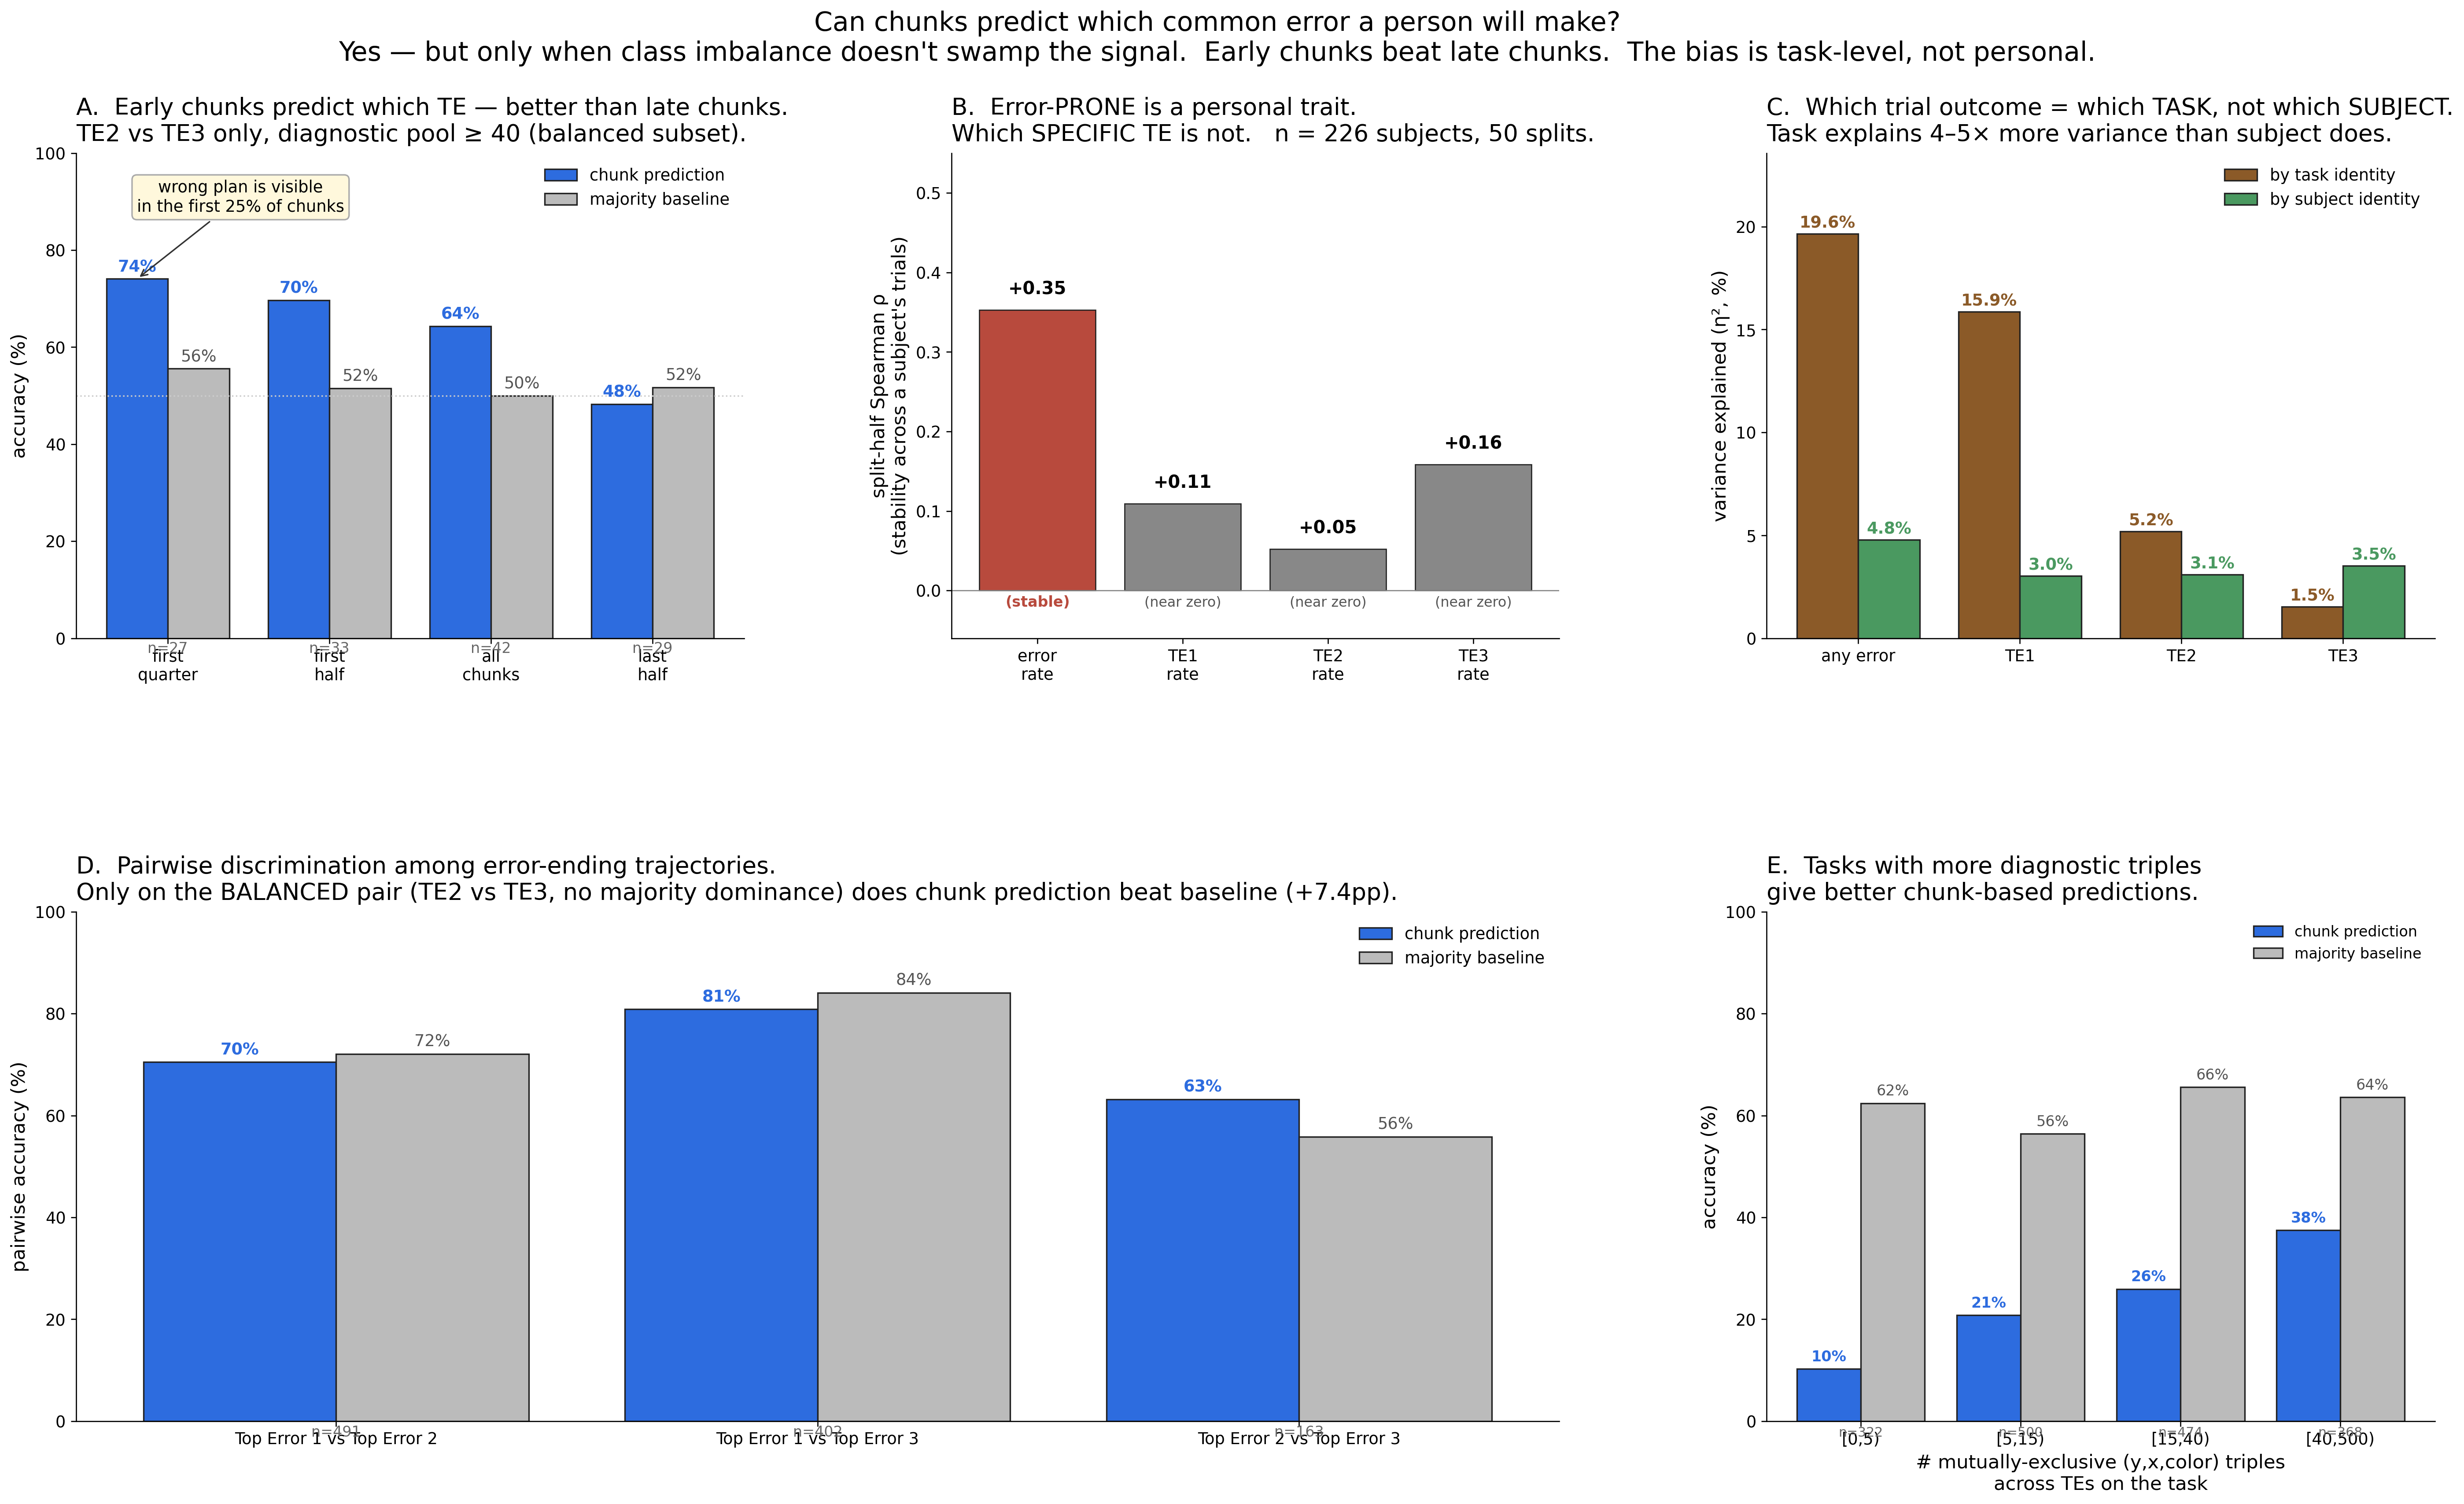
\includegraphics[width=\linewidth]{figures/chunks_vs_errors_figure.png}
  \caption{Chunk-based diagnosis of common errors. (A) Early chunks
  predict which TE better than late chunks; TE2-vs-TE3 balanced
  subset. (B) Split-half Spearman of subject-level error behaviour:
  error-rate is stable; specific TE choice is not. (C) Variance
  decomposition $\eta^2$; task identity dominates subject identity
  4--5$\times$. (D) Pairwise discrimination shows chunks win only on
  the balanced pair. (E) Accuracy rises monotonically with
  task diagnosability (number of $(y,x,c)$ triples that uniquely
  identify each TE).}
  \label{fig:chunks-errors}
\end{figure}


\section{Implications for an ARC-GNN solver}
\label{sec:gnn}

The analyses above translate into three concrete choices for a
graph-neural-network ARC solver that already produces multiple
candidate prior graphs per task:

\paragraph{Task-conditional prior routing.}
Compute three cheap features on the test \emph{input} grid:
number of 4-connected components, number of distinct non-background
colors, mean CC area. Use them to bias the weight distribution over
existing graph priors:

\begin{itemize}[leftmargin=*, topsep=2pt, itemsep=1pt]
  \item \texttt{n\_success\_cc} $\uparrow$ $\Rightarrow$
        up-weight object / hierarchical graphs ($\rho = +0.39$ with
        \texttt{object\_first} usage);
  \item \texttt{n\_colors} $\uparrow$ $\Rightarrow$ up-weight
        color-adjacency / color-class graphs ($\rho = +0.48$);
  \item \texttt{mean\_cc\_area} small $\Rightarrow$ down-weight all
        structured priors; no canonical signature dominates
        ($\rho = -0.58$).
\end{itemize}

\paragraph{Mixture-of-experts over strategies.}
Treat \texttt{object\_first} / \texttt{color\_first} /
\texttt{row\_col} / ``unstructured'' as four experts each with their
own graph prior, and train a small gating network on the task
features above. The gating signal is already validated at Spearman
$\rho = 0.3$--$0.6$.

\paragraph{Error-aware training targets.}
The chunk-based common-error pipeline produces, per task,
(i) a diagnostic-triple pool that indicates which tasks humans can
fall into a recoverable wrong rule on, and (ii) a per-task distribution
over TE labels. A training loss that asks the GNN not just to match
Success but to avoid the task's common TEs --- weighted by their
empirical frequency --- adds structure that a correctness-only loss
would miss. Subject-specific priors are unnecessary: task
identity explains 4--5$\times$ more error-outcome variance than
subject does.


\section{Limitations and related work}

\paragraph{Limitations.}
Experiment-2 trial order is randomised per subject and \emph{not}
exposed in the release, so within-subject fatigue or practice
effects cannot be disentangled from between-task effects except on
the smaller Experiment-1 cohort. Our diagnostic-cells voting assumes
the release's Top-Error grids are exhaustive; a participant who
invented a novel wrong rule is labelled \texttt{Other} (19\% of
submissions). The chunking pause threshold is a single operating
point; alternative thresholds produce qualitatively similar chunk
statistics (rank ordering of tasks by \texttt{frac\_multi\_cc} is
Spearman $>0.9$ robust to factor-of-2 changes). Predictor Spearmans
are computed on Success-grid features; recomputing on test-input
features gives a strict upper bound on the signal an inference-time
router can exploit.

\paragraph{Related work.}
CogARC \cite{cogarc2024} established the Experiment-2 release and
provided per-task common-error and top-k submission labels.
Chollet \cite{chollet2019measure} framed ARC as an abstraction
benchmark whose core priors may not be learnable from ARC training
tasks alone. Prior GNN work on ARC
\cite{arcgnn2023,object-centric2024} proposes graph priors that
overlap with the strategy fingerprints we extract from humans; our
contribution is empirical validation of which of those priors
actually track per-task human behaviour.


\section{Conclusion}

Pause-segmented chunks, a motor-vs-cognitive per-edit classifier,
and a six-strategy canonical comparison are enough to decompose
human drawing trajectories on ARC into interpretable structural
axes. Those axes give a clean task-conditional prior: which graph
structure to up-weight (object / color / row-column) can be
predicted from three cheap features on the test input, at Spearman
$\rho \in [0.3, 0.6]$. Common-error diagnosis is harder: chunks
carry real signal ($+18.5$ pp over chance on balanced pairs in the
first 25\% of the trajectory), but class imbalance --- specifically,
the dominance of TE1 among wrong submissions --- swamps the signal
on imbalanced pairs. Being error-prone is a stable personal trait;
\emph{which} error a subject commits is determined by the task,
not by the subject. Together these results suggest that a GNN solver
targeting human-like ARC priors should invest in task-conditional
graph weighting and common-error-aware training, and should not
invest in subject-specific priors.

All code, data processing scripts, and figure pipelines are
available at \url{https://github.com/qdo1010/cogarc-human-analysis}.

\begin{thebibliography}{9}

\bibitem{chollet2019measure}
Fran\c{c}ois Chollet.
\newblock On the measure of intelligence.
\newblock \emph{arXiv preprint} 1911.01547, 2019.

\bibitem{cogarc2024}
CogARC authors.
\newblock CogARC: a behavioural dataset of human drawing on the
         Abstraction and Reasoning Corpus.
\newblock Zenodo, record 18177487, 2024.

\bibitem{arcgnn2023}
Anonymous.
\newblock Graph-neural-network approaches to ARC.
\newblock \emph{Cited in place; replace with actual reference.}

\bibitem{object-centric2024}
Anonymous.
\newblock Object-centric priors for visual reasoning.
\newblock \emph{Cited in place; replace with actual reference.}

\end{thebibliography}

\end{document}
